%%%%%%%%%%%%%%%%%%%% author.tex %%%%%%%%%%%%%%%%%%%%%%%%%%%%%%%%%%%
%
% sample root file for your "contribution" to a contributed volume
%
% Use this file as a template for your own input.
%
%%%%%%%%%%%%%%%%%%%% author.tex %%%%%%%%%%%%%%%%%%%%%%%%%%%%%%%%%%%

\RequirePackage{fix-cm}

% RECOMMENDED %%%%%%%%%%%%%%%%%%%%%%%%%%%%%%%%%%%%%%%%%%%%%%%%%%%
\documentclass[smallextended]{svjour3} 

% Choose options for [] as required from the list in the Reference Guide

\usepackage{mathptmx} 	% selects Times Roman as basic font
\usepackage{helvet} 		% selects Helvetica as sans-serif font
\usepackage{courier} 		% selects Courier as typewriter font
\usepackage{type1cm} 		% activate if the above 3 fonts are
								% not available on your system

\usepackage{makeidx} 		% allows index generation
\usepackage{graphicx} 	% standard LaTeX graphics tool

% when including figure files
\usepackage{multicol} 						% used for the two-column index
\usepackage[bottom]{footmisc} 			% places footnotes at page bottom
\usepackage{amsmath,amssymb,epsfig}
\usepackage{epstopdf}
\usepackage{multirow}
\usepackage{colortbl}
\usepackage{longtable} 
\bibliographystyle{spmpsci}

% See the list of further useful packages in the Reference Guide
\smartqed  % flush right qed marks, e.g. at end of proof

%\makeindex 	% used for the subject index
				% please use the style svind.ist with
				% your makeindex program

% RECOMMENDED %%%%%%%%%%%%%%%%%%%%%%%%%%%%%%%%%%%%%%%%%%%%%%%%%%%

% Use the package "url.sty" to avoid problems with special characters used in your e-mail or web address
\begin{document}
%\title{Gaze-based control of robot-swarm using electroencephalography} % Fix!
%\title{EEG-based proximal interaction between humans and groups of robots}
%\title{EEG-based implicit communication between human and robots}
\title{Electroencephalography as implicit communication channel for proximal interaction between human and robot swarm}
%\title{Proximal interaction between an operator and a group of robots based on electroencephalography} % Fix!

\titlerunning{EEG as implicit communication channel for proximal interaction between human and swarm}% for an abbreviated version of your contribution title if the original one is too long

\author{Luca Mondada \and
	Mohammad Ehsanul Karim  \and
	 Francesco Mondada}
%\authorrunning{L Mondada, M E Karim and F Mondada}

% Use \authorrunning{Short Title} for an abbreviated version of your contribution title if the original one is too long

\institute{Luca Mondada \at
	Department of Physics, Swiss Federal Institute of Technology ETHZ, Z\"urich, Switzerland \\
	\email{lmondada@ethz.ch}
	\and
	Mohammad Ehsanul Karim \at
	Laboratoire de Syst\`emes Robotiques, Ecole Polytechnique F\'ed\'erale de Lausanne, Lausanne, Switzerland \\
	\email{ehsan.mce@gmail.com}
	\and
	Francesco Mondada \at
	Laboratoire de Syst\`emes Robotiques, Ecole Polytechnique F\'ed\'erale de Lausanne, Lausanne, Switzerland \\
	\email{francesco.mondada@epfl.ch}
	} % Fix!

\date{Received: date / Accepted: date}

\maketitle

% @lucacomment "such techniques are not very intuitive". I'm not sure we can say that as some of those techniques do aim at being as intuitive as possible...
\begin{abstract}

Search and rescue, autonomous construction, and many other multi-robot semi-autonomous robotics applications can benefit from an efficient interaction between an operator and a group of robots. 
%Among the possible control schemes, some take advantage of a shared environment between human and robot and are based on proximal interactions. 
When interacting with a swarm of robots, it could be interesting for the operator to follow the rules of swarm interaction, supporting the scalability and the robustness of the swarm by having only local proximal interaction and sharing the physical environment of the robots.
Most research on proximal interaction with groups of robots has studied gesture and speech recognition to select the robots among the group or to give orders. 
Such explicit communication techniques require specific conventions in gestures or speech that need to be learned and can be culture-dependent. 

This study proposes a new \textit{implicit} proximal communication technique to approach the problem of robot selection. We use electroencephalography (EEG) signals to select the robot the operator is looking at. This is achieved using the steady-state visually evoked potential (SSVEP), a repeatable neural response to a regularly blinking visual stimulus that varies predictively based on the blinking frequency. In our experiments, the robot was equipped with LEDs blinking at different frequencies, and the operator's SSVEP neural response was extracted from the EEG signal to detect and select the robot. This study systematically investigates several factors that directly impact the efficiency of the system in the specific case of a human - multiple robot interaction. In particular, we study several parameters impacting on the SSVEP neural response: distance between the robot and the operator, the LED color, and the LED blinking frequency. Based on these parameters, we study two signal processing appraoches and critically analyze their performance on 10 subjects controlling a set of physical robots. 
Our results show that despite the numerous artifacts, it is possible to achieve a recognition rate higher than 85\% on some subjects, the average on ten subject being at 75\%.

\keywords{human-robots interaction \and EEG \and SSVEP \and Emotiv EPOC \and Thymio robot}
\end{abstract}

\section{Introduction}
\label{sec:introduction}
Swarm robotics has extremely promising applications, such as search and rescue, environmental monitoring, autonomous construction, or geographic mapping. 
The topic has been extensively studied under various perspectives: swarm robotics \cite{brambilla2013}, collective robotics \cite{kernbach2013handbook}, or distributed robotics \cite{martinoli2012distributed}, depending on the form of interaction among the robots. 
To date, researchers and engineers have successfully designed scalable \cite{rubenstein2012kilobot}, robust \cite{winfield2006safety}, efficient (compared to single robot) \cite{Bonani2012}, and affordable distributed multi-robot systems \cite{rubenstein2014programmable}. 
On top of the challenge in designing autonomous control strategies, researchers have recently shown an increasing interest for another aspect of swarm robotics: human-robot interaction. 
Although many single-robot control interfaces have shown interesting results, human-swarm interaction (HSI) is still a state-of-the-art problem~\cite{Kolling2016}. \\
%In this paper we will use the acronym HRsI (\textit{robot} pluralized) to define human-robot interaction with groups of robots, these being swarms or simply multiple individual robots.\\
\\
A majority of researchers addressing the interaction with a robot swarm use remote control strategies, based on a centralized approach allowing the operator to have an overview of the mission~\cite{Kolling2016}. 
This approach contrasts with several basic principles of swarm-robotics, relying on simple mechanisms, local interactions and spatially targeted communication, among others. 
These principles, normally applied to robots only, can also be considered for human-robot interaction.
This is possible, for instance, when human and robot swarm share the same physical environment. 
In these situations, the operator can have a local interaction with the part of the swarm close to him/her, and can observe the same environment that the robots observe. 
In the literature, this interaction is called \textit{proximal}, in opposition to \textit{remote} interactions~\cite{Kolling2016}.\\
\\
%Triggering the interaction with a specific robot can either allow the operator to control a robot working independently within a group or to control a swarm, for instance through a leader~\cite{Goodrich2012}.
We therefore consider an application scenario where an operator is surrounded with mobile robots that have semi-autonomous behavior. This can be for instance the case of an inspection or construction task. 
The operator simply interacts with the robots that are close to her/him and share the same environment. The robots can be either acting independently or be part of a swarm. 
In our application scenario, when the robots meet a predefined condition, find some interesting information, or cannot solve an issue, they stop and request a command from the operator. In the case of a swarm, the robots stopping and asking for interaction with the operators could be either single agents or could be leaders of a sub-group of the swarm~\cite{Goodrich2012}. As several robots can be in this situation, the operator has to select one of them, based on criteria that are application dependent and managed by the operator himself. Triggering the interaction of a single robot within a group is a challenging HSI problem: we need to use a communication channel easily accessible to the operator, combined with an infrastructure that is distributed and compatible with the swarm robotics approach.
Fong et al. have proposed a simple selection protocol that uniquely identifies each robot using a numbering system; the selection and manipulation of the robots were performed via a remote control \cite{fong2003}. 
Such systems require several explicit coding rules that add on top of the communication channel, reducing efficiency and being incompatible with a distributed system. 
Various other more intuitive methods, such as gesture recognition \cite{Couture-Beil2010,Jones2010,Monajjemi2013,Nagietal2014}, robot-vision-based user-gaze interpretation \cite{Couture-Beil2010,Monajjemi2013,Pourmehr2013}, and speech recognition \cite{Pourmehr2013} have been studied. 
There are several relevant literature reviews on the topic \cite{goodrich2007human,Kolling2016,yanco2004classifying}.\\
\\
Most of the aforementioned methodologies have been tested on real robots. 
For example, automated vision-based detection of hands and face combined with machine learning-based spatial gesture analysis showed successful selection of a single drone from a group of four just by robot vision. 
The research team claimed that their algorithm can scale up to 20 drones \cite{Nagietal2014}. Similar research discussed the capacity of vision-based systems considering varying distance between the operator and the robot; in particular, the studied range was 1 to 4\,m~\cite{Couture-Beil2010}. 
However, speech and gesture interaction systems have some practical limitations: (1) they require prior training of the operator to specific coded words or gestures that can be culture-dependent~\cite{Trovato2013}, limiting intuitive interaction~\cite{Kirchner2015};
(2) they are sensible to the detection of the intention to interact, as they use communication channels that are common with other tasks~\cite{Rzepecki2012}; (3) they are based exclusively on explicit communication, generating heavy protocols~\cite{Kirchner2015}.\\
\\ 
To address these issues, we studied the use of electroencephalography (EEG) signals to address the robot selection problem. 
This approach does not require the definition and learning of explicit communication codes, as it is based on the implicit information extracted by EEG of the operator observing the robot. 
We define \textit{implicit information} as provided by the operator in a passive way, in opposition to \textit{explicit} information exchanged actively~\cite{Kirchner2015}.
We define \textit{implicit communication} as an exchange of \textit{implicit information}.
EEG-based implicit communication is not culture-dependent, and EEG techniques are more reliable than gesture and speech-based techniques in detecting the intention to interact~\cite{Rzepecki2012}.
Recent advances in neuroscience provide us with reliable and affordable devices that allow acquisition of two reliable and well-documented EEG neural responses -- the P300 and the Steady-State Visually Evoked Potential (SSVEP) \cite{Beverina2003,Bi2013,Zhu2010}. 
The P300 neural response is elicited as a reaction to salient stimuli. 
The SSVEP, on the other hand, is measured when a visual stimulus is repeatedly shown at a certain frequency. Although the P300 response has been given more attention, recent studies show that target selection can be achieved efficiently using SSVEP since it is possible to distinguish reliably multiple SSVEP responses corresponding to different frequencies through computational analysis \cite{SSVEPfiability}.
Therefore, we used SSVEP and lights blinking at different frequencies in our robot selection scenario to detect the target being watched by the operator. This suggestion of a new communication channel is compatible with the swarm robotic paradigm but does not solve the question of the distributed infrastructure, that will not be addressed in this paper. For this layer of HSI we refer the reader to the last results in protocols implementing spatially targeted communication~\cite{mathews2015spatially}.\\ 
\\ 
The SSVEP response can be extracted from an EEG signal following several approaches~\cite{Bi2013}. 
Most studies use machine learning based on linear discriminant analysis (LDA), but this approach requires a training phase that we want to avoid, to validate the fact that we use pure implicit communication.
Therefore we decided to apply two other techiniques: a signal processing approach using canonical correlation analysis (CCA), and a simpler short-time Fourier transform (STFT).
The CCA-based approach has been chosen because it does not require training and showed very interesting results on the same equipment we used in our study~\cite{Lin2014}.
The simple short-time Fourier transform (STFT)~\cite{Durak2003} has been chosen because of its relative simplicity and fast response. The delay of the response of the system is probably the major limitation of most SSVEP-based approaches.\\
To obtain the best possible results, we started our study by exploring the role of three key parameters of the system: the distance between the operator and the robot, the color of the visual stimuli, and the frequency of the blinking light. 
Once the optimal parameters set, we tested our approach on ten subjects, most of them without experience in using EEG-based interfaces. \\
\\
This paper is structured as follows. Section \ref{sec:soa} presents a state of the art in SSVEP-based brain-computer interfaces (BCI). Section \ref{sec:methods} gives further details about the experimental setup and, in particular, about the EEG device, the robot, and the general data-collection protocol. 
Section \ref{sec:prestudy} presents the study on the three key parameters of our set-up: the color, the frequency, and the distance of the targets. Section \ref{sec:CCA_approach} build on the chosen parameter to study the performances on ten subjects of the CCA and STFT approaches. A discussion section concludes the paper.

\section{State of the art}
\label{sec:soa}
After the pioneering example of BCI for the control of a wheelchair by Millan et al.~\cite{millan2004noninvasive}, the research community has shown a growing interest for this mobile robot interaction technique~\cite{Bi2013}. The main motivation behind these studies is to enable severely disabled people to control wheelchairs. With a better understanding of these techniques, other usages have appeared, including the control of mobile robots by healthy subjects in various applications. The work by Kishore et al.~\cite{kishore2014comparison}, targeting the control of a humanoid robot, is a representative example of the most common approach: the interaction is made through a screen, where all possible commands are associated with visual stimuli~\cite{Volosyak2009}. When the subject looks at a given command on the screen, the associated stimulus frequency is detected in the EEG signal and the command is triggered. Stawicki et al.~\cite{Stawicki2016} follow the same approach using a screen, but illustrate the commands in an interface based on the subjective view of the robot, coming from a camera located on the mobile robot itself. A slightly more sophisticated approach consist in introducing an avatar to represent the possible actions~\cite{Faller2010}. An additional abstraction can be introduced by having the selection of an goal that can be achieved by a combination of actions, for instance by selecting the destination in the scenario of driving a car~\cite{Fan2015}. Most BCI studies targeting the control of mobile systems follow this same approach, having a computer screen as support for the visual stimulus~\cite{Bi2013}. Computer screens offer a lot of flexibility in the graphical expression of the commands and in the placement of the stimuli. \\
\\
G{\"{u}}neysu et al.~\cite{Guneysu2013} control a humanoid robot with a panel of LEDs instead of a computer screen. Although the principle of displaying a set of possible commands on a LED matrix is identical to the one using computer screens, the choice of LEDs allows a better flexibility in the choice of frequencies. Also Ortner et al.~\cite{Ortner2010} use LEDs on a control panel to define the direction of a mobile robot, but have a specially designed shape for their panel, better fitting its purpose. Still, none of these studies allows a direct proximal interaction with the robot, always introducing a control panel between user and robot. To our knowledge, only Jacobs~\cite{Jacobs2013} studied a direct interaction, with the visual stimuli created by LEDs on the robot itself. In his study, the LEDs are placed at the end of three arms fixed on the robot. The three arms correspond to three directions (forward, right, and left) that the user can choose by looking at the corresponding LEDs. This work was very preliminary and tested on very few subjects.\\
\\
Concerning the choice of the neural response to be used to detect the intention of the user, SSVEP is increasignly chosen as it is usable by most people~\cite{Guger2012}. SSVEP-based target selection procedures allows to choose among many items. Gao et al.~\cite{SSVEPfiability} claimed that their algorithm could successfully detect 45 different target frequencies using green blinking LED lights. The performances of SSVEP-based systems can be improved by coupling them with other neural responses, like the P300~\cite{yin2015hybrid}. In the domain of rehabilitation, the combination of SSVEP and P300 signals has been used to control actual wheelchairs~\cite{paper4}. These performances come at a cost: they require EEG acquisition systems that are extremely expensive and not portable, and experiments in conditions that are extremely controlled.\\
\\
The goal of reaching practical applications pushed the development of affordable and portable EEG headsets, but most consumer headset have less than five electrodes and do not allow to explore a sufficiently large number of signals. Only two affordable systems acquire signals on 14 or 16 electrodes: the OpenEEG and the Emotiv EPOC headsets. The OpenEEG is an affordable system targeting research experiments~\cite{Salehuddin2011}, but requires an important deployment effort. The Emotiv EPOC is simpler to deploy~\cite{jian2014improving,van2012designing}; Compared to traditional systems that require gel on the scalp as well as cumbersome wiring, Emotiv uses saline water and a radio connection. However, ease of use and affordability come at the price of poorer signal quality. Still, a comparative analysis of SSVEP data acquired from EPOC and medical-grade EEG found that the data is reliable \cite{liu2012implementation}, although researchers advised not to use Emotiv for medically serious cases \cite{duvinage2013performance}. The radio connection is also a limitation, but studies have shown its reliable use in real-time applications~\cite{hvaring2014comparison}.\\
\\
Our goal is to explore the use of neural responses for proximal interaction with a swarm of robots, without a computer screen or a panel of LEDs between robots and operator. The choice of the SSVEP as neural response seems obvious, as well as the choice of he Emotiv EPOC headset. Because of the novel configuration of use, based on the generation of stimuli directly on the robot body, the choice of several parameters was less trivial. \\
The LED blinking frequency is the first critical parameter. The blinking frequencies used in the literature vary in a range from 4.5\,Hz to 50\,Hz~\cite{Zhu2010}. However, since the signal to noise ratio in EEG is higher in the lower part of the spectrum, some researchers have suggested using low frequencies for SSVEP-based applications \cite{paper6}.\\
The distance between the target and the operator is another critical parameter. Wu et al.~\cite{wu2013effect} have studied the impact of distance on the SSVEP response, but using only one stimulus, and therefore not studying the impact in a scenario with a choice.\\
The color is a third key parameter. In the literature, white was predominantly preferred over red, green, or blue \cite{paper6,aljshamee2014beyond,aljshamee2016discriminate,cao2012flashing,paper2}. Cao et al. justified the preference: white is a combination of all the primary colors and therefore excites cone-cells associated with red, green, and blue simultaneously \cite{cao2012flashing}. 
Some studies, however, have successfully used red \cite{Faller2010,jian2014improving,paper4} and green \cite{chua2004effects,duvinage2013performance,SSVEPfiability,hvaring2014comparison,paper4,mouli2013performance} stimuli as well. Some studies observed even red to be more effective than white \cite{Faller2010,hvaring2014comparison}, while others found green to be more effective under similar comparative conditions \cite{chua2004effects,duvinage2013performance}. 
There is also contradictory evidence between the red and green colors; Mouli et al. observed green to be more effective \cite{mouli2013performance}, while others were more successful using red~\cite{cao2012flashing}. Therefore we decided to conduct our own study on the impact of color of stimuli on our SSVEP response detection.


%Considering Emotiv EPOC, red stimuli was empirically observed to be more effective than white \cite{hvaring2014comparison}.
%Finally, the time needed by the operators in most target selection setups is, in general, at least 3\,s~\cite{Fan2015,SSVEPfiability,jian2014improving,paper4}.
%In some cases (here in real driving conditions), the target selection process can take up to 26\,s~\cite{Fan2015}.

\section{Material and methods}
\label{sec:methods}
For the acquisition of EEG signals, we used the Emotiv EPOC EEG headset \cite{stytsenko2011evaluation}. 
As described in Section \ref{sec:soa}, this headset is a good tradeoff between affordable price and level of performance. 
It is affordable with respect to medical-grade devices; however it is expensive (approximately \$700 with drivers to access raw data) compared to other ``consumer'' headsets because of its 14 electrodes (see Figure \ref{fig:electrodes} for their positioning on the skull), allowing several types of data acquisition. 
%This and other aforementioned features are sufficient to allow for meaningful research experiments. 
A final advantage is its compatibility with open-source EEG signal acquisition and processing software for BCI design. This study uses OpenViBE, a well-established open-source BCI design software \cite{ov_publication}.\\
\\
\begin{figure}
\center
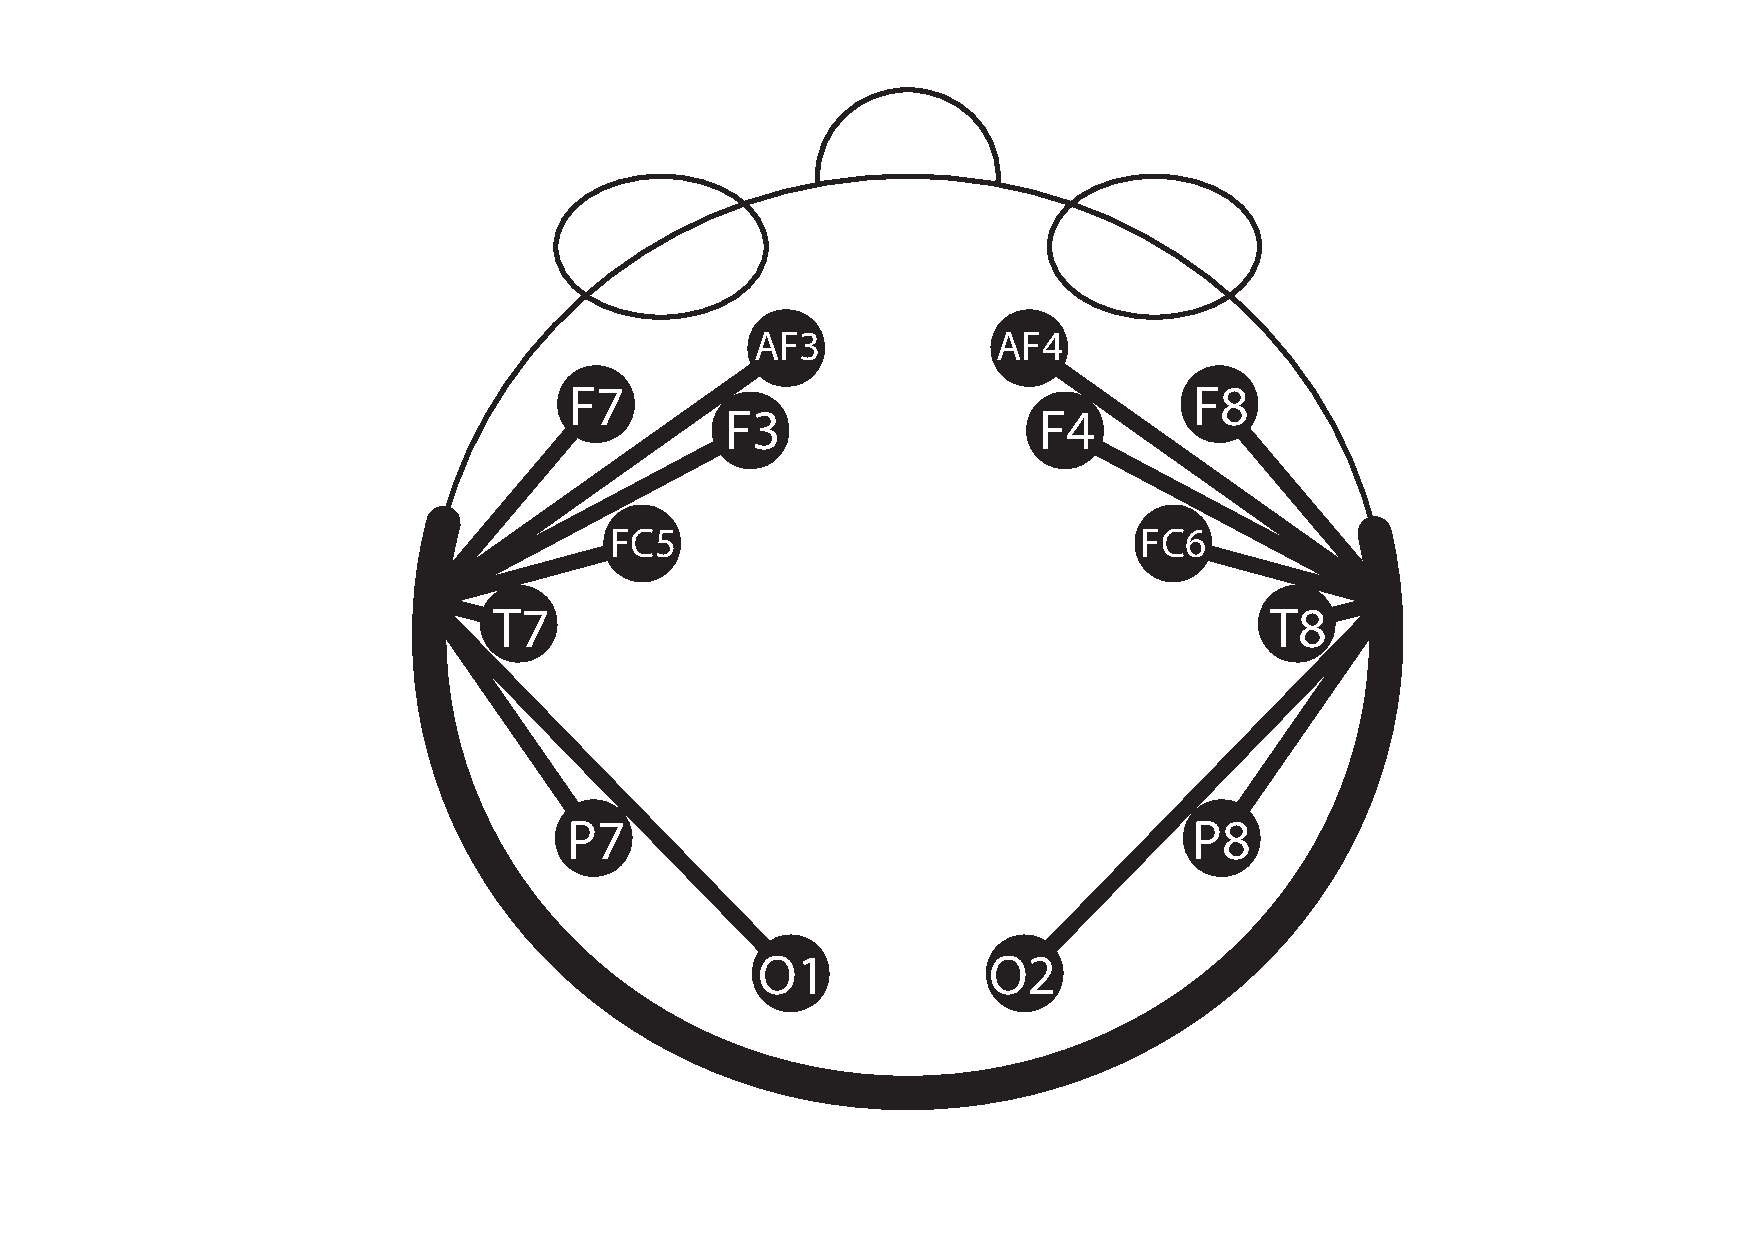
\includegraphics[width=0.5\textwidth]{figures/emotiv-electrodes.pdf}
\caption{Top view of the location of the electrodes of the EMOTIV EPOC EEG headset on the skull (forward looking direction toward the top of the image), with their international code labeling.} \label{fig:electrodes}
\end{figure}
\\
As the robot for our experiments, we used Thymio II; this programmable robot features a differential drive system, infrared (IR) remote control receiver, and LEDs to change body color \cite{Riedo-et-al-2013}. Its small size ($11 \times 11 \times 5\,\mathit{cm}$) and affordable price (approximately \$130) make it well suited for multi-robot experiments. 
The communication between the computer and the robot was supported by an infrared emitter dongle controlled by USB. 
In this configuration, the computer only plays the role of the processing and communication unit of the operator, establishing local communication with the robots that are in the field of view of the operator.\\
\begin{figure} \center
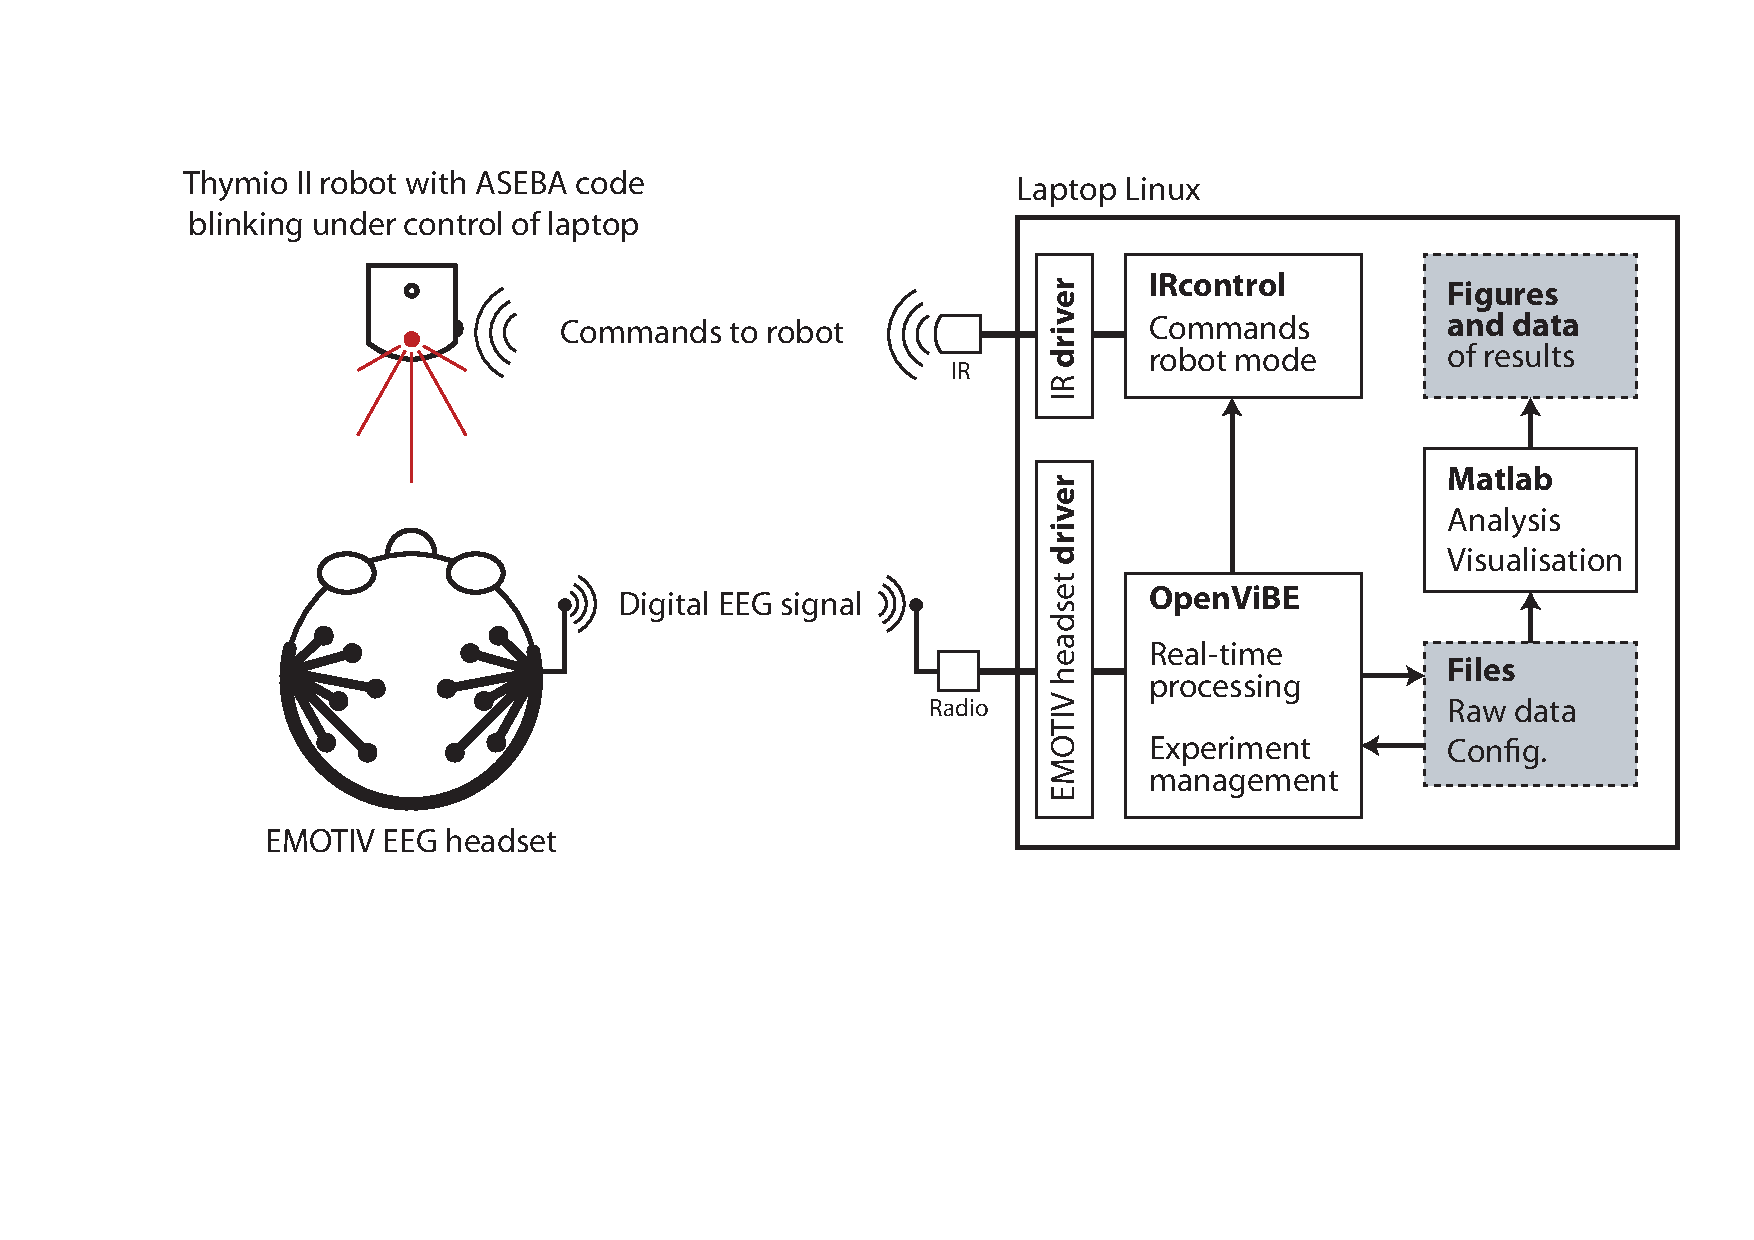
\includegraphics[width=\textwidth]{figures/schema-global.pdf}
\caption{Configuration of the experiment: the left side illustrates the spatial arrangement of the experiment; the right summarizes the signal acquisition and the processing method.} \label{fig:thymioinstall}
\end{figure}\\
\\
Figure \ref{fig:thymioinstall} summarizes the experimental setup. 
The subjects were placed in front of three robots. 
Each experiment was composed by a set of trials. In each trial, the subjects were instructed to look at an indicated target robot. 
One second after the instruction, all three targets began to flicker for 7\,s. During the stimulus, the subjects were asked to look at the blinking light; moreover, they were requested to blink as little as possible to limit EEG artifacts. 
A break of 3\,s was then introduced to avoid tiring the subject. 
%This process was repeated eight times for each target frequency plus a neutral non-blinking condition. \\
%Finally, to reward the subjects, we implemented a visualization where the successful recognition is displayed on the robot's LEDs by turning them green as soon as the classification has been made, and then making the chosen robot controllable by a remote control.\\

\section{Preliminary study: parameter optimization}
\label{sec:prestudy}
%This section provides details about the experimental setup and the data-collection protocol used for collecting data to test on the LDA-based algorithm \cite{openvibeSSVEP}.\\

To optimize the extraction of the SSVEP within the EEG signal, we studied the impact on the strength of the SSVEP response of three important interaction parameters: blinking frequency, blinking color, and distance to the stimulus. 
These studies do not only make sense within the context of HSI but also have more fundamental scientific interest. 
To our knowledge, these parameters have not been systematically studied, and in particular in a situation where the stimulus is generated on the robot body. We only know from generic EEG literature that the recognition reliability decreases if either the frequency or the distance to the stimulus target increases~\cite{herrmann2001,wu2013effect}. 
Concerning the color of the stimuli, we know that the color white can emit three times as much light as red, green, or blue and stimulates all three cone cells in the eye, which could potentially lead to stronger neural responses \cite{aljshamee2016discriminate,cao2012flashing}. 
However, existing literature states that ``it is difficult to decide which color is the best'' for SSVEP~\cite{Zhu2010}.
Finally, the impact of these parameters for the acquisition of data in our experimental conditions is unknown. 
%Given the reduced signal acquisitive capability of the Emotiv EPOC device as compared to standard medical-grade EEG headsets, we expect the limits to be significantly lower.\\
\\
\subsection{Evaluation metrics}

To evaluate the quality of the SSVEP response, we computed a metric that indicates how prominent the stimulus frequency is in the EEG signal.
To compute this metric, we applied the fast Fourier transform to the EEG signal of a each trial to obtain the frequency spectrum. 
To quantify the detectability of the SSVEP, we used the \textit{first peak to the second peak ratio} (FSR)~\cite{Zheng2010}:
given a particular frequency $f$, let $F$ and $R$ be two disjoint subsets of the averaged spectrum such that $F$ contains the spectrum of the frequencies $[f-1, f+1]$, and $R$ contains the frequency range $[6, f-1[ \,\cup\, ]f+1, 24]$; the FSR ratio is then defined as:
\begin{equation}
\label{recog_rat}
q =:\frac{\max F}{\max R}
\end{equation}
\\
The FSR provides the ratio of the highest peak within $[f-1, f+1]$ to the highest peak in the rest of the spectrum. 
The neural response to a regularly blinking stimulation, called SSVEP, is characterized by a peak in the spectrum of the signal at the same frequency as the blinking frequency. 
Thus, if the FSR based on the stimuli frequency is above 1, then the highest peak is within 1\,Hz of $f$, and the SSVEP can be considered detectable and recognized. 
Otherwise, the SSVEP cannot be observed. 
We therefore call $q$ the \textit{recognition ratio}.
Please note that we decided to consider peaks up to 1\,Hz off from the stimulation frequency as valid SSVEP responses because we always have at least 2\,Hz difference between one stimulation frequency and another. 
This band could be restricted, as existing literature shows that neural responses are, in general, very accurate~\cite{SSVEPfiability}.

\subsection{Parameter: Stimulation frequency}
% @lucacomment Here we have a serious problem: the definition of the recognition ratio goes up to 18Hz whereas we apparently make measures up to 24Hz, which does not make much sense...
% I don't know if it was my mistake at the time of plotting (I hope not!) or if it is a writing mistake...
Six frequencies were tested (9, 12, 15, 18, 21, and 24\,Hz). For each frequency condition, five trials were performed on three different subjects. The subjects had normal or corrected-to-normal vision and no history of major head injury. The blinking light was set 1\,m away from the subject. 
Figure \ref{fig:graph-frequences} confirms the decrease in the amplitude of the neural response as the frequency grows as already described in the existing literature~\cite{herrmann2001}; furthermore, it shows that the detection fails beyond 15\,Hz. 
This is lower than what was observed in the literature with medical-grade EEG headsets; in \cite{SSVEPfiability}, the range used is 6 to 24\,Hz. Therefore, we deduced that SSVEP activity can be measured with this headset and in these physical conditions, but provided that low frequencies are chosen.
Based on these observations, we restricted the frequency band in the following two studies; the chosen interval was [7\,Hz, 17\,Hz].

\begin{figure}
\center
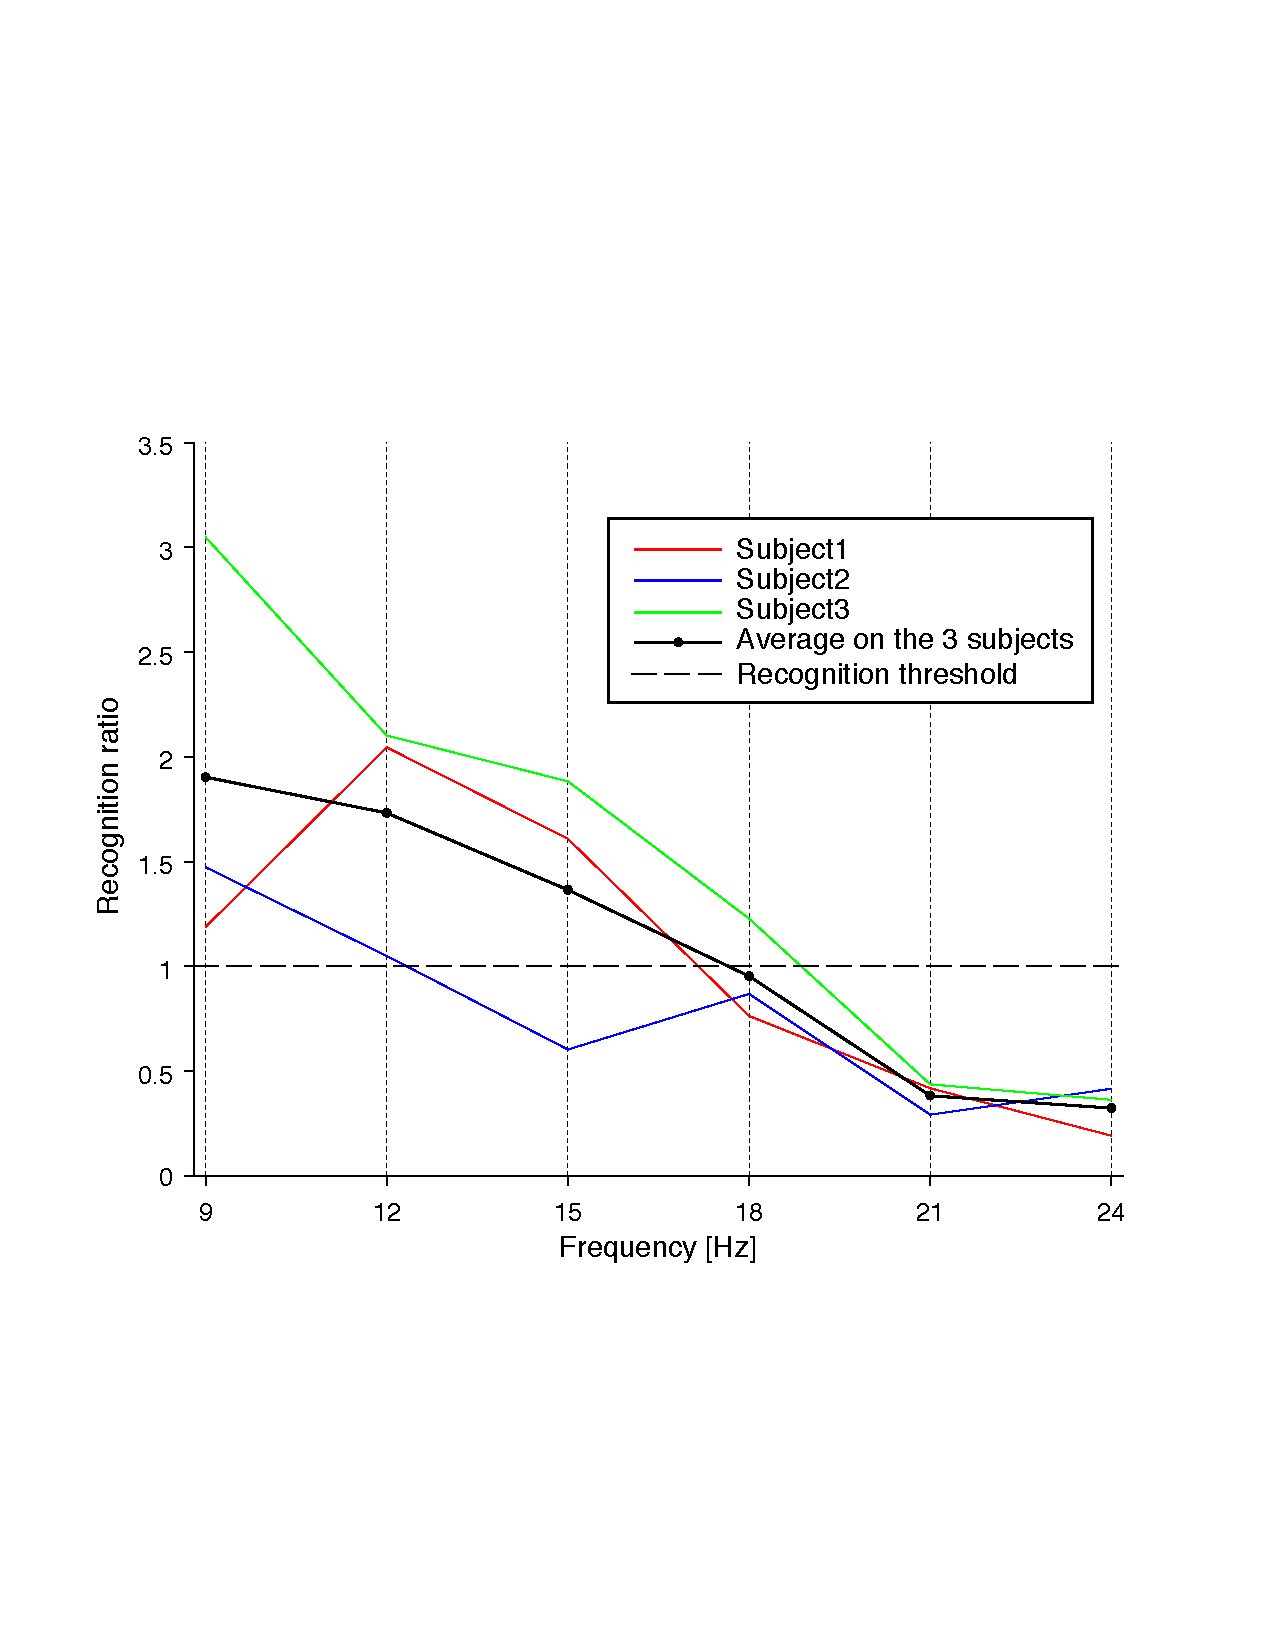
\includegraphics[width=0.8\textwidth]{figures/graph-frequences.pdf}
\caption{Recognition of a red visual stimulus in the EEG spectrum based on its blinking frequency. Each of the three subjects has been subjected to five trials for each frequency; the trial period is 7\,$s$. The plotted recognition ratios for each frequency represents the values of the averaged power spectrum of the five stimulation trials.} \label{fig:graph-frequences}
\end{figure}

\subsection{Parameter: Stimuli distance}
As a second parameter, we analyzed the impact of varying distance between the operator and the blinking target robots, taking into consideration each of the frequencies: 7, 9, 12, 15, and 17\,Hz; the tested distances were: 30\,cm, 1\,m, and 2\,m. 
Considering the small size (12\,cm in diameter) and the weak light emitting power of the robot ($<$ 300\,mW electrical power), these experimental distances correspond to a range of 1.5\,m to 10\,m for a robot of a diameter of 60\,cm with a 7.5\,W light, corresponding to a standard LED lamp. 
This range seems compatible with the proximal interaction of a operator directly in contact with the robot. For a distance larger than 10\,m, the perception of the environment by the operator cannot allow a shared consideration of the environment. This maximal distance is also compatible with a local communication infrastructure between the robot and the equipment of the operator.\\
The experiment was conducted on three subjects, where on each subject we performed four trials for each frequency and each distance. 
Figure \ref{fig:graph-distances} summarizes the results; there is not much difference in neural response between 30\,cm and 1\,m; however, the response starts to deteriorate at 2\,m. Indeed, the recognition ratio at 2\,m falls under 1.0 at 13\,Hz. 
The reasons are: (1) the targets become smaller with increasing distance and (2) the LED light intensity deteriorates, leading to a weaker SSVEP response.

\begin{figure}
\center
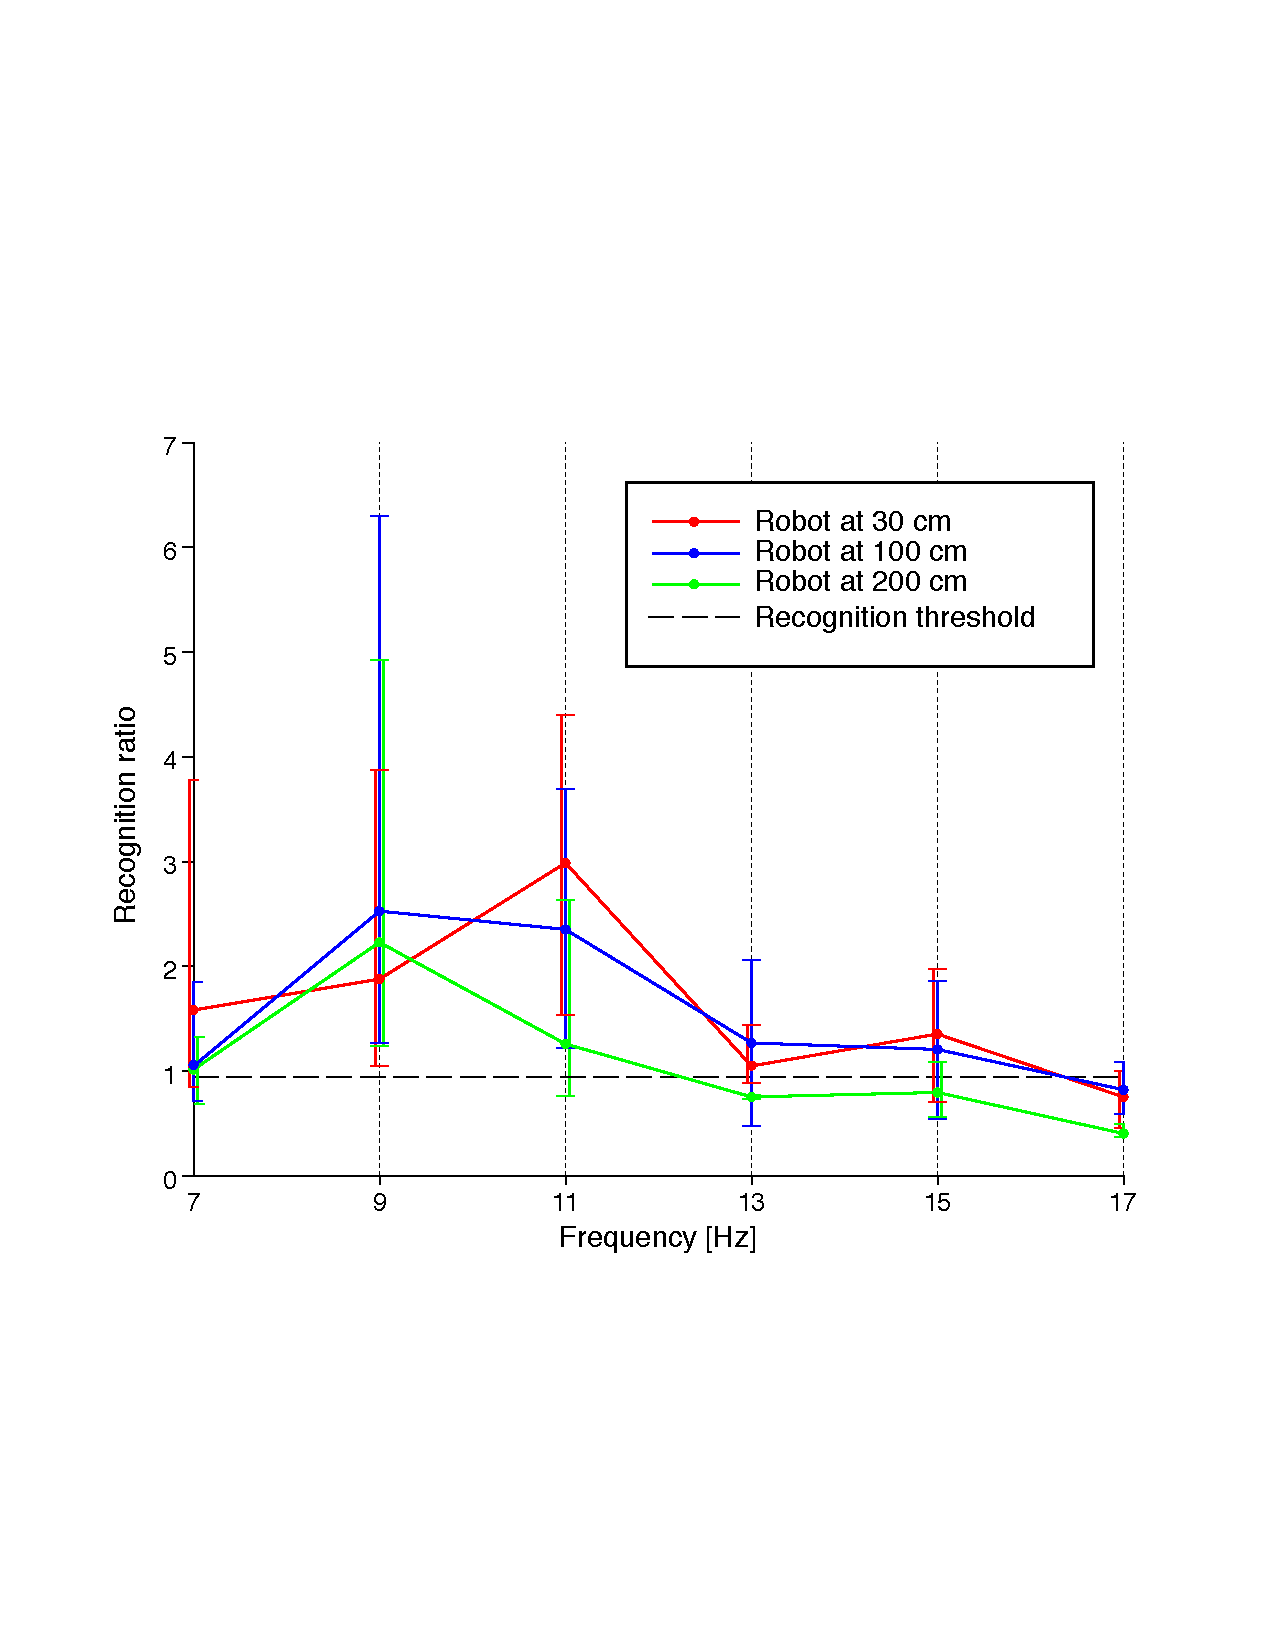
\includegraphics[width=0.8\textwidth]{figures/graph-distances.pdf}
\caption{Recognition of a red visual stimulus in the EEG spectrum based on the distance of the robot. Four trials per subject for each distance and frequency combination was performed. The plotted recognition ratio for each frequency and distance combination represent the values of the averaged power spectrum of all the stimulation trials on all the subjects.}
\label{fig:graph-distances}
\end{figure}
%Fixed!
\subsection{Parameter: Stimulation color}
The experiment featuring stimulus color was similar to the stimulus-distance one. Four trials were conducted for each combination of frequency (7, 9, 12, 15, and 17\,Hz) and LED color (red, green, and white). The target robot was at 1\,m from the subjects. Figure \ref{fig:graph-couleurs} shows that the best results were obtained using the red or green stimuli, which conforms to part of the literature \cite{chua2004effects,duvinage2013performance,Faller2010,hvaring2014comparison}. Moreover, white color does not increase the neural response; therefore, our results contradict the findings of Cao et al. as documented in \cite{cao2012flashing}. 

\begin{figure}
\center
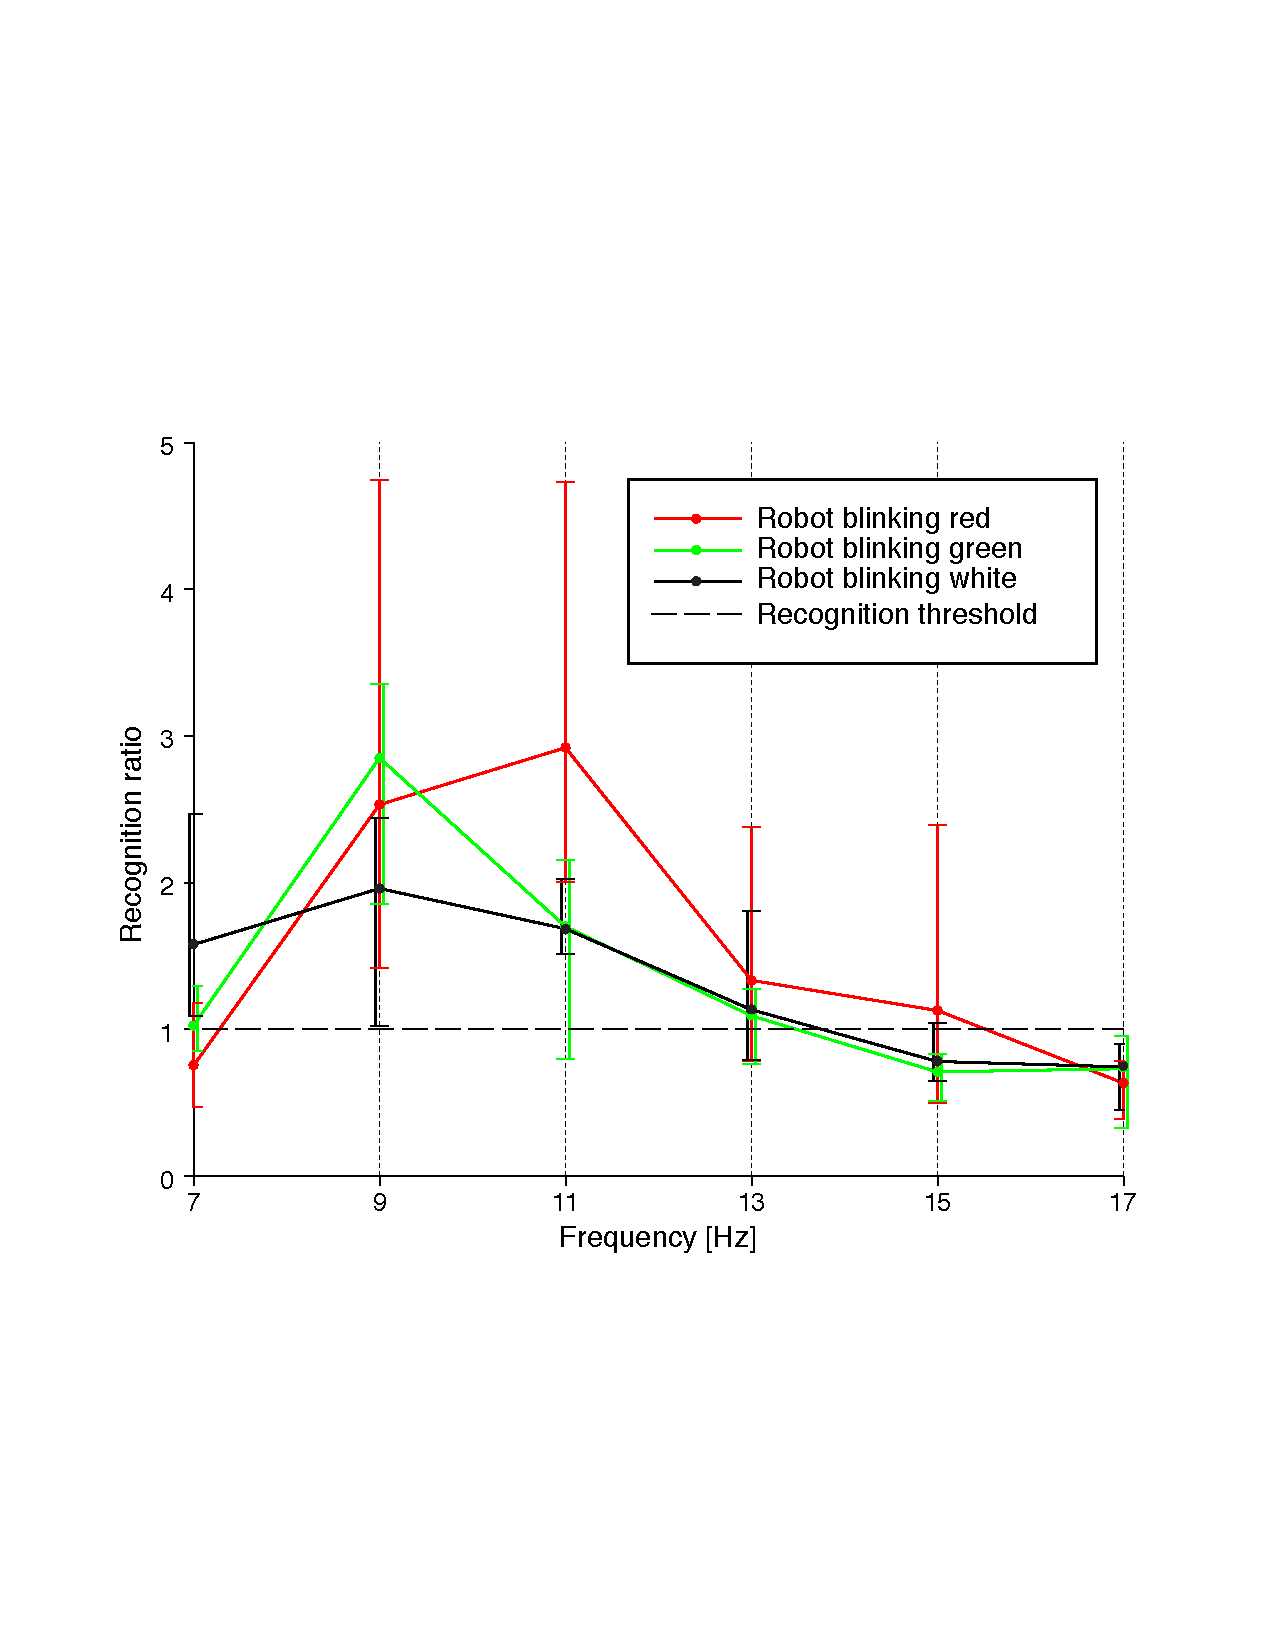
\includegraphics[width=0.8\textwidth]{figures/graph-couleurs.pdf}
\caption{Recognition of a visual stimulus in the EEG spectrum based on its color. Four trials per subject for each color and frequency combination were performed. The plotted recognition ratios for each frequency and distance combination represent the values of the averaged power spectrum of all the stimulation trials on all the subjects.} \label{fig:graph-couleurs}
\end{figure}

\section{Robot selection by SSVEP response}
\label{sec:CCA_approach}

Based on the results of the studies described above, we designed an experiment to implement and test the robot selection methodology using CCA-based and STFT-based SSVEP analysis. The schematics of this setup can be found in Figure \ref{fig:experiment-set-up}. 
Three Thymios blinking in red at frequencies of 8, 10, and 12\,Hz are placed in a half circle, 90 degrees apart.
In addition to the general architecture presented in Figure~\ref{fig:thymioinstall}, we equipped the subject with an IR remote control.
The subject looks at the robot she/he wants to control, and the EEG signals acquired from the Emotiv device are used to make a prediction with the processing chain.
This information is transmitted via IR to the robots.
The selected robot turns green and executes the command received from the IR remote control while the other robots remain red and ignore these commands.\\
\\
The subjects were exposed to 15 trials: 5 trials at each frequency. Before each trial, the subjects were told which of the three robots she/he should look at and was given 4\,s to prepare. During the trial, the subject had to look only to one robot even though all three robots were blinking; a 3\,s break followed each trial.
To assess the reliability of this methodology, the experiment was conducted on 10 different subjects, mostly with no previous experience with EEG.
The subjects were aged between 17 and 48: three women (age: 17, 32, and 44) and seven men (age: 18, 18, 19, 29, 35, 37, and 48). 

\begin{figure}
\center
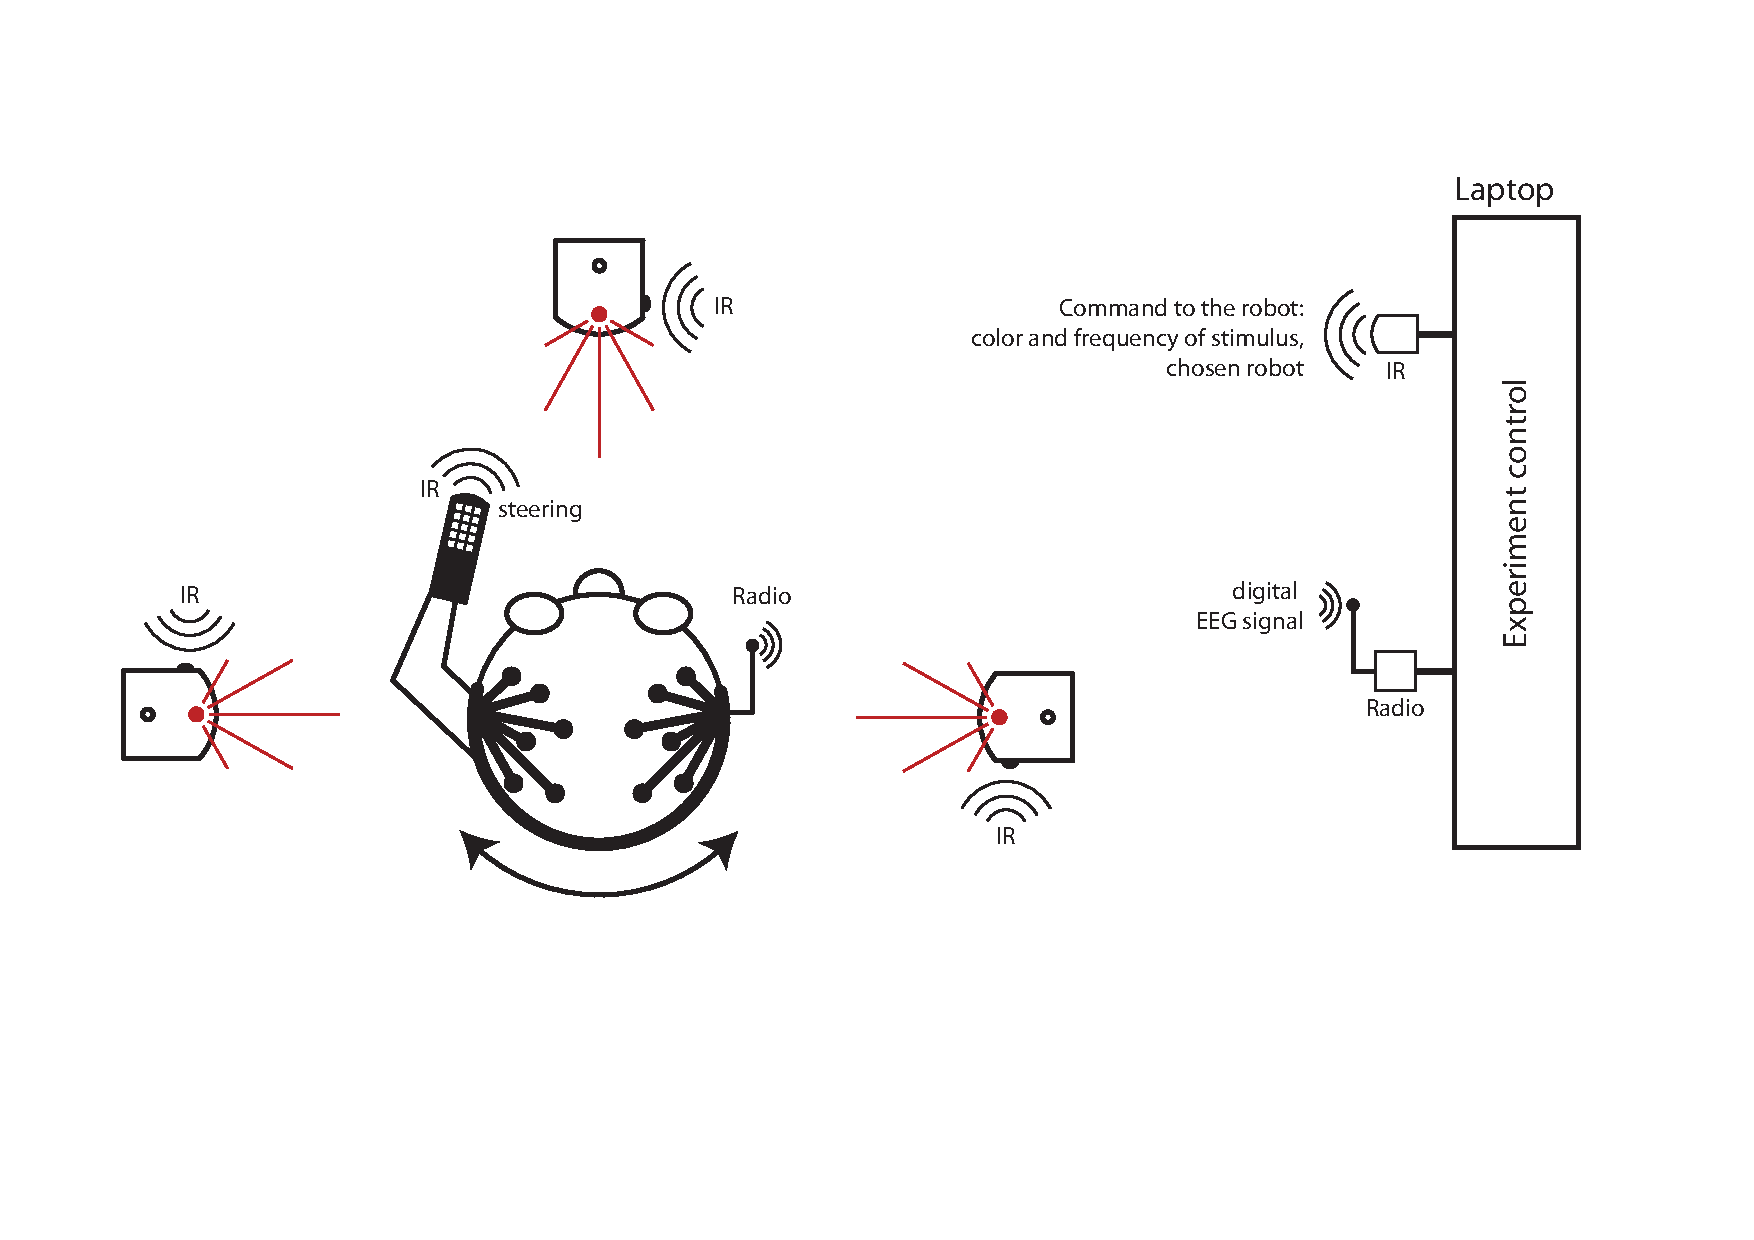
\includegraphics[width=0.9\textwidth]{figures/schema-global2.pdf}
    \caption{Setup of the experiment, showing the configuration of the subject with respect to the robots and the communication channels used for interaction. The detailed schematics of the computational unit (signal acquisition and processing chain) are the same as shown in Figure \ref{fig:thymioinstall}.} \label{fig:experiment-set-up}
\end{figure}

\subsection{Signal processing}

Figure \ref{fig:schema-openvibe-cca} shows the details of the signal processing chain.
The objective of the signal processing method used in this study is to classify the SSVEP response from the occipital region of the brain (O1 and O2) into one of the following three categories: 8\,Hz, 10\,Hz, and 12\,Hz.
This region of the brain is known to be neurologically important in the SSVEP process, as it contains most of the visual cortex.
The signal processing consists of a loop that is repeated until a successful classification can be made.
After each unsuccessful iteration, a signal length parameter is increased. Initially this parameter is set to 2\,s.
It represents the length of the signal that is used during the classification attempt.
In the event of classification failure, a new attempt is made with a signal length increased by 0.25\,s.
This increased length boosts the chances of success of the new classification attempt by reducing the impact of the noise present in the signal
but at the same time introduces longer recognition delays as changing states do not affect the predictions as quickly as before.
If the signal length parameter reaches 8\,s, the classification is interrupted and no prediction is made.
Each loop iteration ends with a classification attempt.
A classification is considered successful only if four consecutive classification attempts have made the same prediction. This measure significantly reduces the false positives and the choice of four consecutive attempts is based on the results of Lin et al.~\cite{Lin2014}.

During each iteration, the classification attempt is made using CCA: the measured EEG signal is correlated with three other signals that are precomputed, and then the signal frequency with the highest correlation to the measured signal is chosen.
The CCA can be thought of as a generalization of the correlation measure to multivariate signals, and has shown good results in SSVEP recognition~\cite{Lin2014}. The principle of this approach is as follows: given two multivariate signals $X$, $Y$, the optimization problem of CCA is to find $\rho$ such that
\\
\begin{equation}
\label{rho}
\rho = \max_{a, b \in \mathbb R^n} r_{ a^\top X, b^\top Y}
\end{equation}
Here, $r_{a^\top X, b^\top Y}$ is the correlation between $a^\top X$ and $b^\top Y$. This is achieved when $a$ is the eigenvector associated to the largest eigenvalue of $S(X, X)^{-1} S(X,Y) S(Y, Y)^{-1} S(Y, X)$; and $b$ is a similar eigenvector of $S(Y, Y)^{-1} S(Y, X) S(X, X)^{-1} S(X, Y)$, where $S(X, Y)$ is the covariance matrix. The proof can be found in \cite{rencher2003}.

In our case the multivariate signals are precomputed models of an idealized reaction to one of the three different blinking stimulations (blinking frequencies of 8\,Hz, 10\,Hz and 12\,Hz).
For a given stimulation frequency, the model is composed of the sine, cosine and the first harmonic of that frequency.
Indeed, SSVEP signals are characterized by amplitude peaks in the frequency spectrum at the respective blinking stimulation.
Using linear combinations of these multidimensional signals, phase, and amplitude as well as superposition of harmonics known to be present in SSVEP signals~\cite{herrmann2001} can thus be modulated arbitrarily to model the SSVEP response of the brain and maximize the correlation with the measured signal.

\begin{figure}
\center
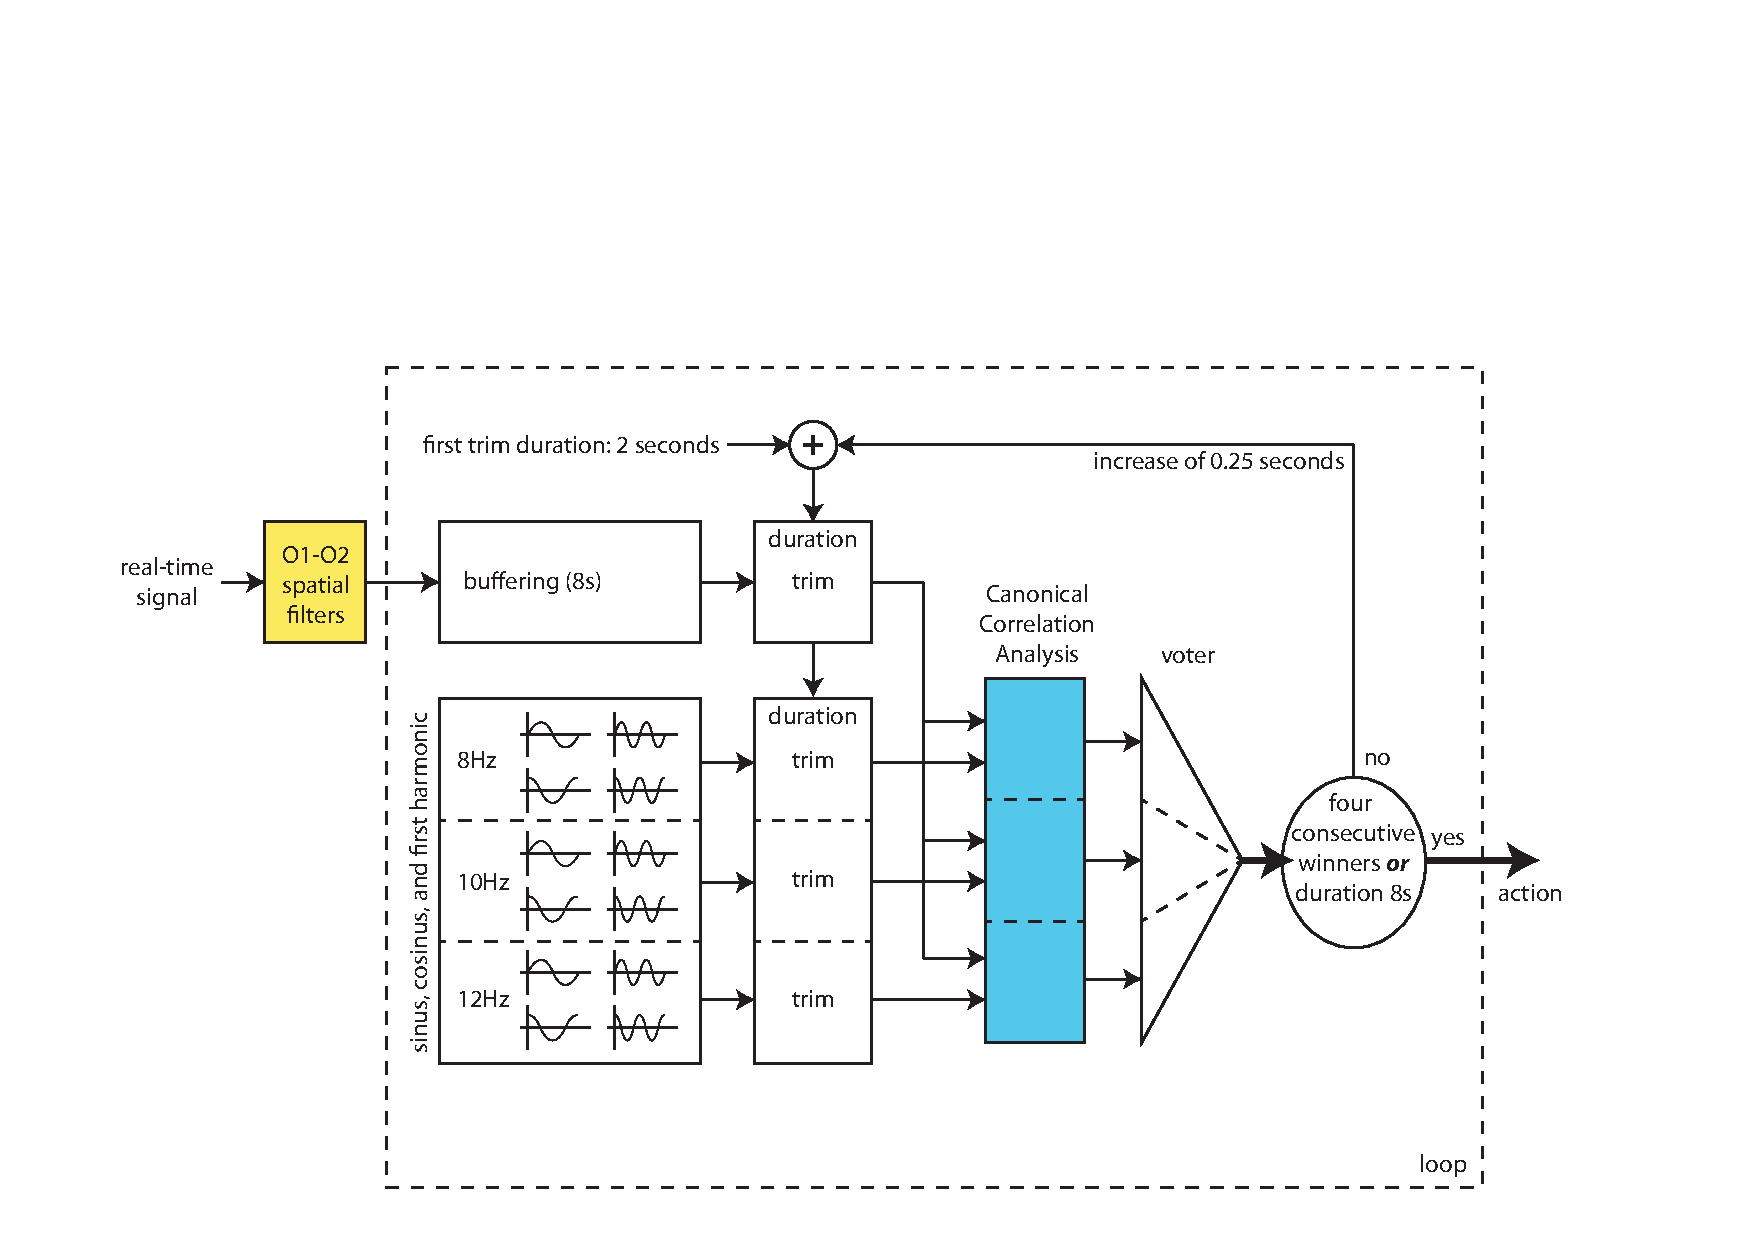
\includegraphics[width=0.9\textwidth]{figures/schema-openvibe-cca.pdf}
\caption{The signal processing chain uses the occipital signals O1 and O2. These signals are first buffered; only the last part of the buffer is used for processing. The length of this period is variable and increased at each processing loop. The signal is compared with ideal signals and the best fit is selected. Four consecutive coinciding predictions are required to have a final selection. The loop is terminated when such a selection is made or when the whole buffer of 8\,s has been used.}
\label{fig:schema-openvibe-cca}
\end{figure}

For comparison, we apply to the same signals a standard STFT~\cite{Durak2003}. 
Starting at the beginning of a stimulation period, the STFT was computed using time frames as long as possible (up to 4\,s) using the available signal, since longer time frames give higher spectrum resolution. %, which is key to limiting the impact of EEG noise.
We therefore used a time frame of 0.5\,s during the first second, of 1\,s in the second second, of 2\,s up to the fourth second, and then a time frame of 4\,s.


\subsection{Results and discussion}
Figure \ref{fig:all_time_reconn} shows the recognition rate as a function of time; the data presented was averaged over all predictions made on all 10 subjects in all stimulations.
It can be seen that the recognition rate starts randomly and increases gradually to plateau around 75\%.
The same increase in recognition reliability after 4\,s can also be seen in Figure \ref{fig:taux-reconn}; this graph shows the average recognition rate per frequency.
We can observe that the lowest reliability is at 12\,Hz, while the highest is at 10\,Hz with very little standard deviation.
The variance between the subjects can be observed in more detail in Figure~\ref{fig:all-results-reconn} and the corresponding Table~\ref{tab:all-results-reconn}; these data show the average recognition rates per subject per frequency.
The predominant reliability of 10\,Hz can be seen in different subjects but especially in Subjects 5 and 7, where the recognition rate at 10\,Hz is double compared to 12\,Hz.
Lastly, this graph also shows the divergences between different people: Subject 1 has a 98\% recognition rate at 8\,Hz, while Subject 5 is around 40\% for the same frequency.
This very high variability is a characteristic of EEG that makes EEG analysis so delicate and must be carefully considered when developing new applications. It is also for this reason that an average of 75\% can be considered as a good result.\\
\\
For comparison, we also computed the STFT on the same data sets.
However, we can see in Figure \ref{fig:all_time_reconn} that the STFT performed significantly worse than CCA.\\
%Its one potential advantage is the possibility to use only much shorter time frames as CCA,
%possibly leading to shorter recognition delays.
%However, in our current scenario, this effect is trumped by its higher sensitivity to EEG signal noise.\\
\\
%Fixed! (ADD REFERENCE)
Based on the results, we can observe that the time required to recognize and select the robot in a reliable way is four seconds. 
Due to the CCA approach and the loop structure of this particular processing process, the first prediction using exclusively EEG signals acquired during the current stimulation can only be made three seconds after the beginning of the stimulation.
An additional second is required to reach the best performances, which matches results achieved in the literature \cite{Fan2015,SSVEPfiability,jian2014improving,paper4}. 
Although this signal processing appraoch does not require a training session, as opposed to systems that use machine learning algorithms, this delay of 4\,s is a clear drawback of this prediction system. 
With further study, this issue could perhaps be addressed using a hybrid processing chain combining the reliability of CCA with the reactivity of STFT.
Nonetheless, the stability of this setup is remarkable: it shows that despite the numerous artifacts, it is possible to achieve, on average, a recognition rate of 75\% at any time after the first 4\,s. \\
\\
%We processed the same data using a short-time Fourier transform (STFT), checking if the frequency extraction could be done in a shorter delay. 
%In the first 5 seconds we therefore applied STFT on 0.5$s$ frames for the first second, on 1$s$ frames for the second second, on 2$s$ frames for the third and fourth second, and on 4$s$ frames for the fifth and sixth second. The results are illustrated in figure \ref{fig:all-results-reconn}. STFT has similar performances then CCA in the first seconds of processing, but does not improve the performances as much as the CCA for longer delays.\\
\\
Finally, we did some preliminary experiments combining the use of EEG signals as illustrated above with some processing of the gyroscope mounted on the EEG headset. 
In our tests we used the lateral movement of the head to trigger the recognition. 
This allows the operator non only to start a recognition by moving the head toward a new target but also to restart the process after a wrong recognition by shaking shortly the head laterally. 
A video illustrating the approach can be accessed at \verb"www.bit.ly/ssvep-bot". 
These preliminary tests improved significantly the whole interaction and show the merit of combining the EEG-based implicit communication with other human-robot interaction methods.

%The small variation also suggests that the prediction system used, as it is, will not provide better results. 
\begin{figure}
\center
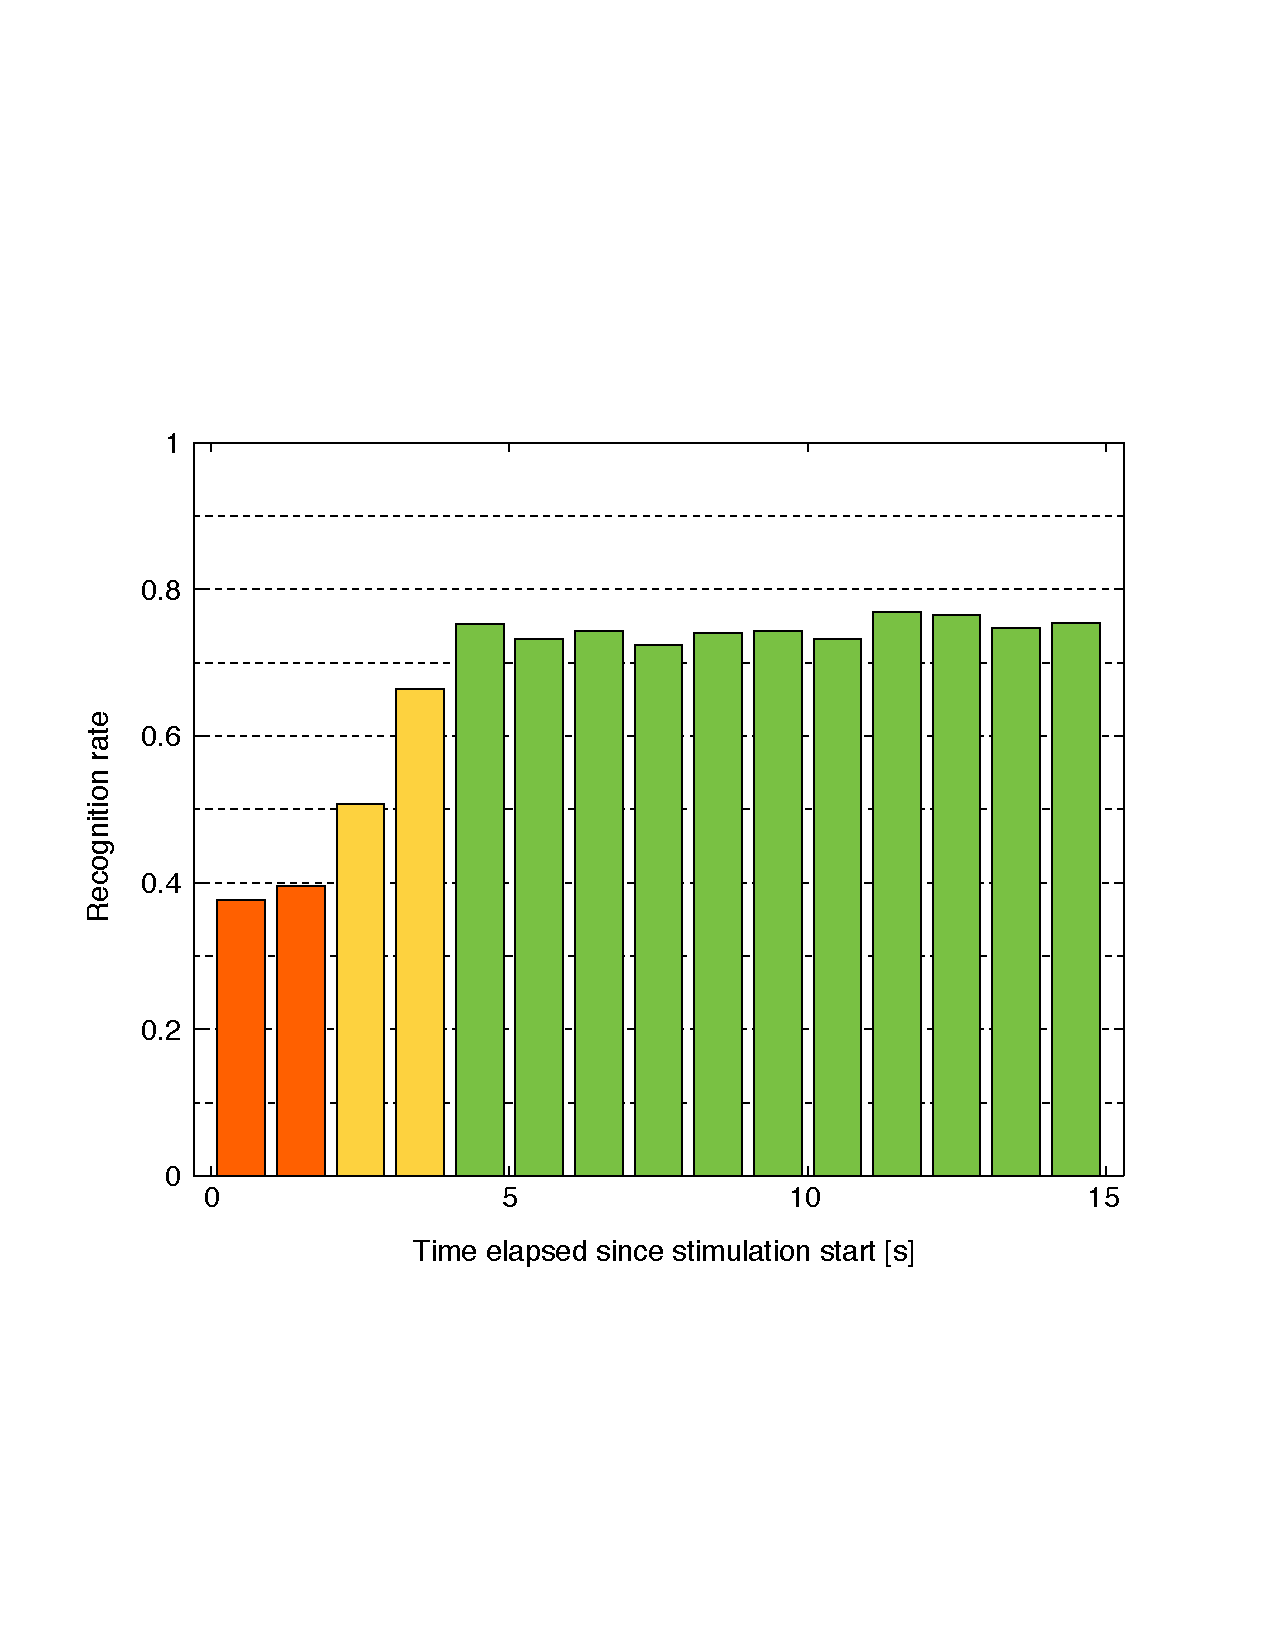
\includegraphics[width=0.7\textwidth]{figures/all_time_reconn.pdf}
\caption{Frequency recognition rate versus time during the 15\,s of stimulation for two processing methods: canonical correlation analysis (CCA) and short-time Fourier transform (STFT). These numbers are an average over 10 subjects considering the 5 trials of 15\,s each and the stimulation frequencies (8, 10, and 12\,Hz).} \label{fig:all_time_reconn}
\end{figure}

\begin{figure}
\center
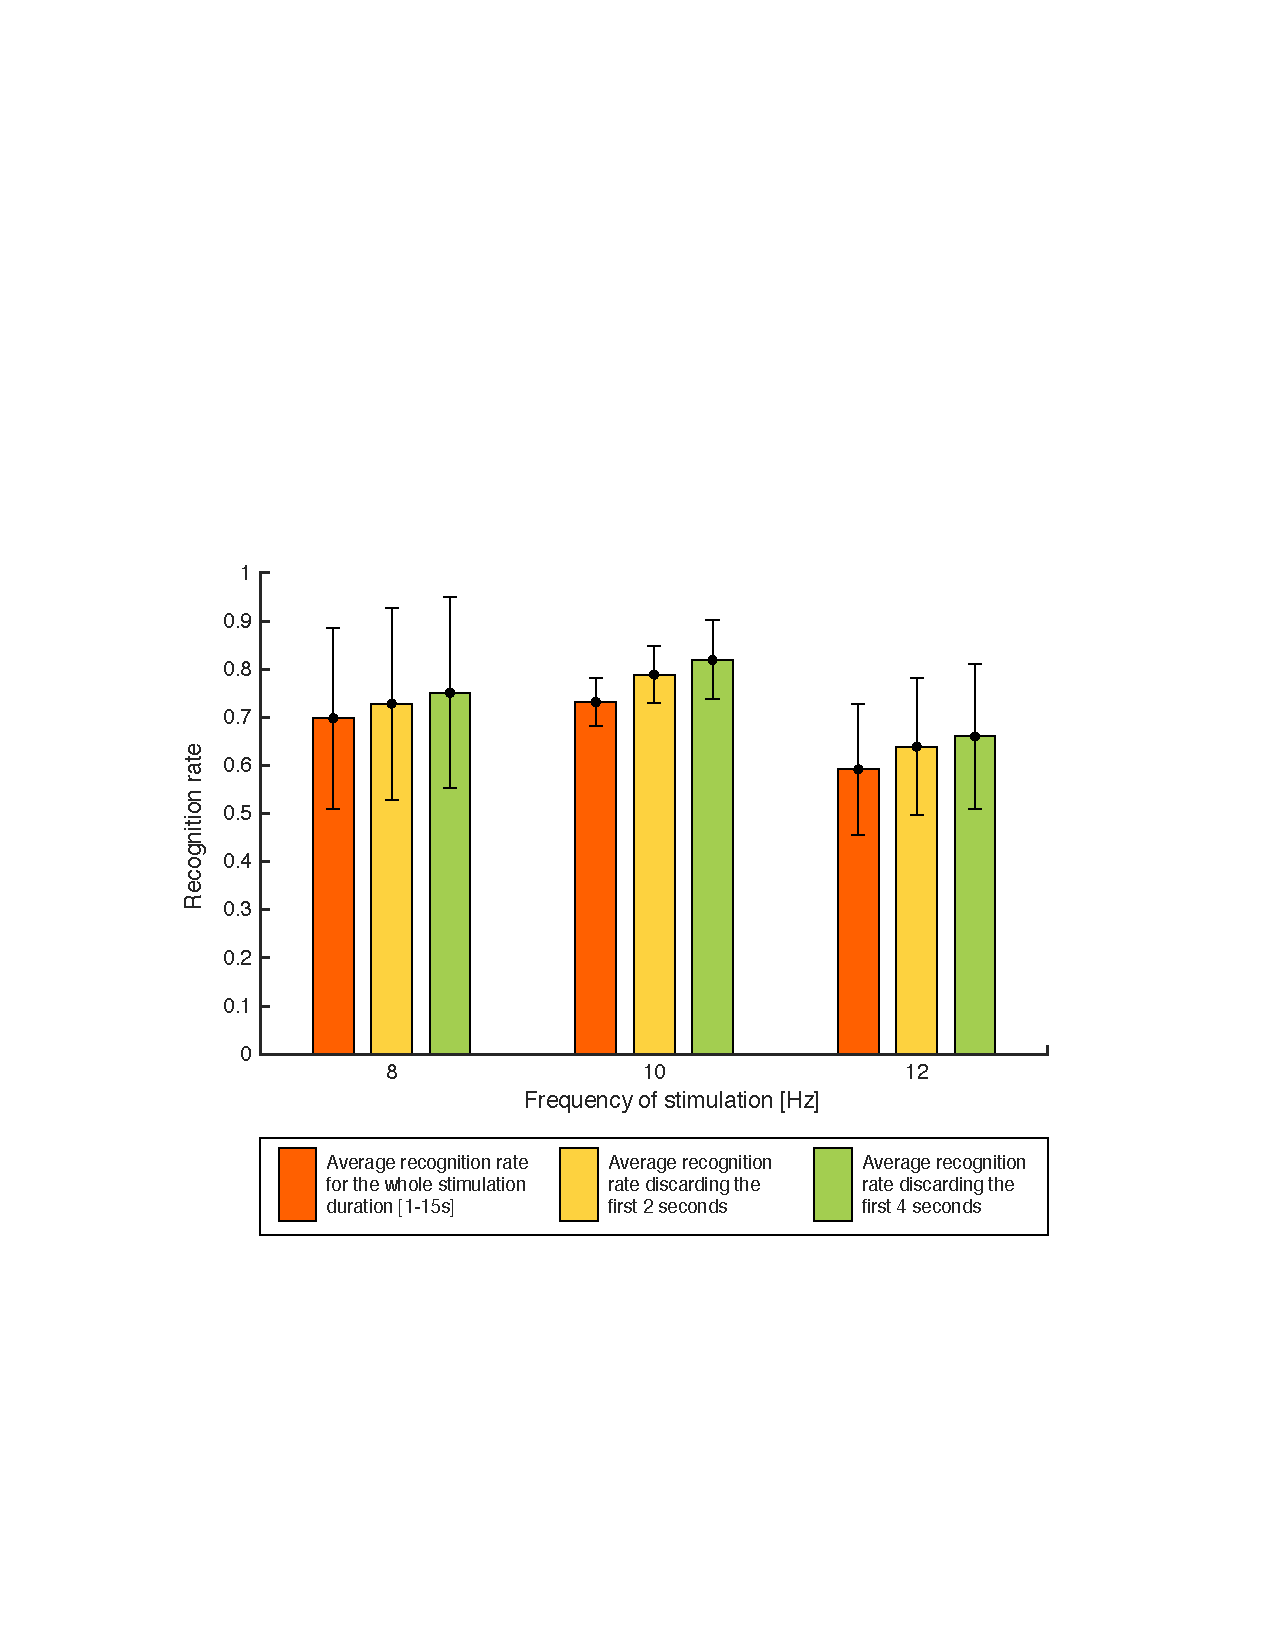
\includegraphics[width=0.7\textwidth]{figures/taux-reconn.pdf}
\caption{Frequency recognition rate per stimulation frequency and per delay between start of stimulation and start of recognition process. These numbers are an average over 10 subjects considering the 5 trials of 15\,s each and the stimulation frequencies (8, 10, and 12\,Hz). The figures for each subject are detailed in Figure \ref{fig:all-results-reconn}.}
\label{fig:taux-reconn}
\end{figure}

\begin{table}\begin{center}
    \begin{tabular}{ c | r | r | r | r | r | r |}
        & \multicolumn{6}{c|}{Recognition rate} \\ 
        & \multicolumn{2}{c|}{delay 0\,s} & \multicolumn{2}{c|}{delay 2\,s} & \multicolumn{2}{c|}{delay 4\,s} \\ 
        Stimuli freq.& average & std deviation & average & std deviation & average & std deviation \\ \hline

         8\,Hz & 69.8\% & 18.8\% & 72.8\% & 20.0\% & 75.1\% & 19.8\% \\
        10\,Hz & 73.2\% &  5.0\% & 78.9\% & 5.9\% & 81.9\% & 8.2\% \\
        12\,Hz & 59.2\% & 13.6\% & 63.9\% & 14.2\% & 66.0\% & 15.1\% \\ \hline
    \end{tabular}
    \caption{Frequency recognition rate per stimulation frequency and per delay between start of stimulation and start of recognition process. These data are plotted in Figure~\ref{fig:taux-reconn}.}
\end{center}\end{table}

\begin{figure}
\center
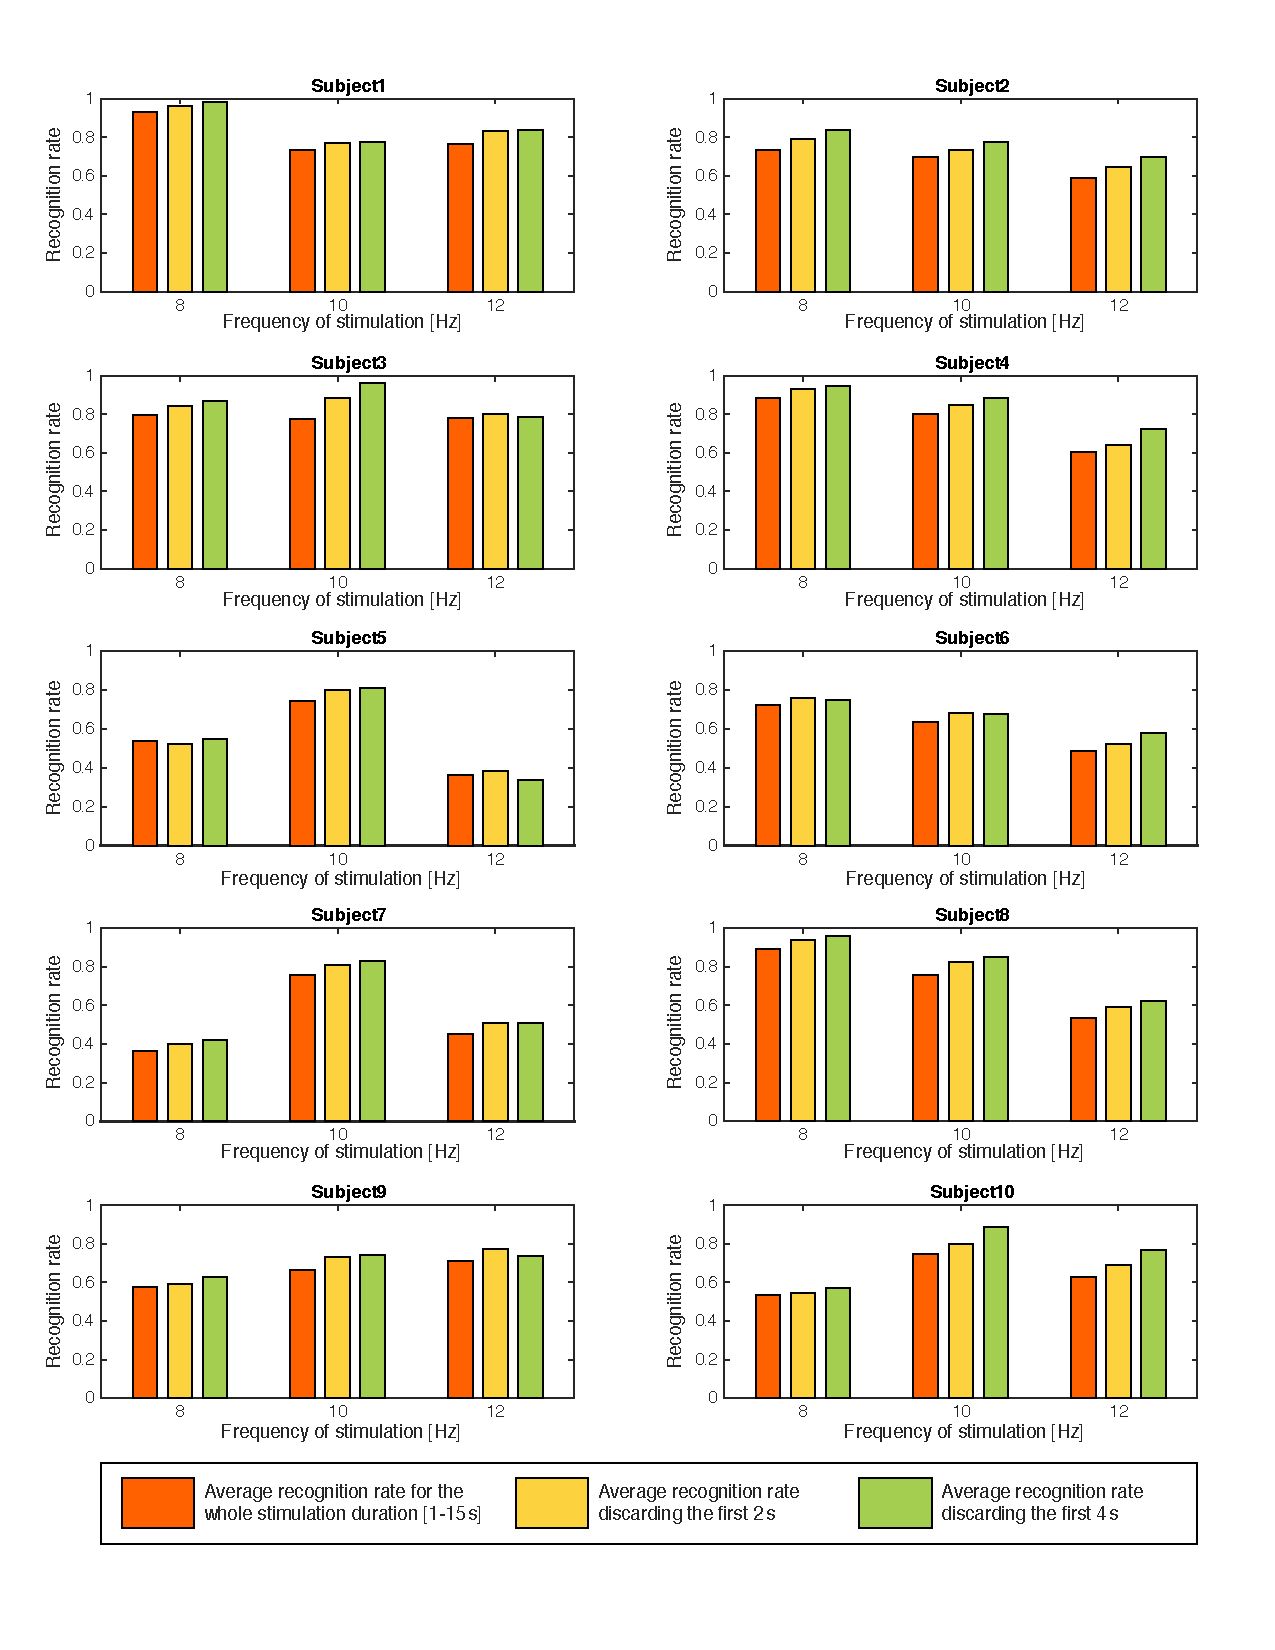
\includegraphics[width=0.98\textwidth]{figures/all-results-reconn.pdf}
\caption{Frequency recognition rate per subject and per stimulation frequency, considering the different stimulation durations. The numerical values are give in Table~\ref{tab:all-results-reconn}.}
\label{fig:all-results-reconn}
\end{figure}


\begin{table}[ht]
\begin{center}
    \begin{tabular}{ r | c | c | c | c || r | c | c | c | c }
        \multicolumn{2}{c|}{} & 0\,s & 2\,s & 4\,s & \multicolumn{2}{c|}{} & 0\,s & 2\,s & 4\,s \\ \hline

        \multirow{3}{*}{subject1} &  8\,Hz & 93.3\% & 96.2\% & 98.2\% & \multirow{3}{*}{subject2} &  8\,Hz & 73.3\% & 79.2\% & 83.6\% \\
                                  & 10\,Hz & 73.3\% & 77.2\% & 77.5\% & & 10\,Hz & 70.0\% & 73.5\% & 77.7\% \\
                                  & 12\,Hz & 76.3\% & 83.1\% & 83.9\% & & 12\,Hz & 58.7\% & 64.6\% & 69.5\% \\
         
        \hline

        \multirow{3}{*}{subject3} &  8\,Hz & 79.7\% & 84.2\% & 86.8\% & \multirow{3}{*}{subject4} &  8\,Hz & 88.6\% & 93.1\% & 94.5\% \\
                                  & 10\,Hz & 77.5\% & 88.5\% & 96.2\% & & 10\,Hz & 80.0\% & 84.9\% & 88.6\% \\
                                  & 12\,Hz & 78.3\% & 80.0\% & 78.6\% & & 12\,Hz & 60.3\% & 64.2\% & 72.3\% \\
        
        \hline

        \multirow{3}{*}{subject5} &  8\,Hz & 53.9\% & 52.5\% & 54.8\% &  \multirow{3}{*}{subject6} &  8\,Hz & 72.4\% & 75.8\% & 75.0\% \\
                                  & 10\,Hz & 74.6\% & 79.8\% & 80.8\% & & 10\,Hz & 63.7\% & 68.4\% & 67.7\% \\
                                  & 12\,Hz & 36.6\% & 38.5\% & 34.0\% & & 12\,Hz & 48.9\% & 52.3\% & 58.2\% \\

        \hline

        \multirow{3}{*}{subject7} &  8\,Hz & 36.3\% & 40.0\% & 41.8\% & \multirow{3}{*}{subject8} &  8\,Hz & 89.0\% & 93.8\% & 95.9\% \\
                                  & 10\,Hz & 75.7\% & 80.8\% & 83.2\% & & 10\,Hz & 75.6\% & 82.4\% & 84.8\% \\
                                  & 12\,Hz & 45.2\% & 50.8\% & 50.9\% & & 12\,Hz & 53.3\% & 59.2\% & 62.3\% \\

        \hline

        \multirow{3}{*}{subject9} &  8\,Hz & 57.8\% & 59.0\% & 62.9\% & \multirow{3}{*}{subject10} &  8\,Hz & 53.7\% & 54.6\% & 57.3\% \\
                                  & 10\,Hz & 66.7\% & 73.4\% & 74.0\% & & 10\,Hz & 74.6\% & 80.0\% & 88.8\% \\
                                  & 12\,Hz & 71.3\% & 77.1\% & 73.7\% & & 12\,Hz & 63.0\% & 69.2\% & 76.8\% \\

        \hline
                                  

    \end{tabular}
    \caption{Frequency recognition rate per subject and per stimulation frequency, considering the different stimulation durations corresponding to the plot of Fig.~\ref{fig:all-results-reconn}}.
\label{tab:all-results-reconn}
\end{center}\end{table}

\section{Conclusions}
This study systematically analyzes two SSVEP classification techniques and some of their key parameters for tackling the robot selection problem in proximal HSI using implicit communication. 
With respect to the existing literature based on other proximal communication such as explicit gestures or voice, this approach uses implicit information that is not culture-dependent and does not require prior learning. On the other hand the SSVEP approach depend on the operator's brain activity, which is very variable from subject to subject. This results in subjects having success rates higher than 85\%, with a peak success rate of 98.2\% on specific frequencies. These performances can be compared with the success rates of other approaches such as gesture- or speech-based HSI~\cite{Nagietal2014,Pourmehr2013}. This variability indicates that some subjects will perform poorly as operator of these interfaces, or will need training to get better performances.\\
\\
Although in gesture- and speech-based interactions the distance is a parameter that is considered when evaluating the success-rate, this is the first study studying the impact of distance on the recognition among several sources of the SSVEP neural response.
Despite the limited range observed in our experiments, less than 2\,m, this distance has to be considered with respect to the size of the robot and the type of visual stimuli. We consider that the setup used in this experiment is equivalent to a robot with a diameter of 60\,cm placed up to 10\,m away and having a blinking LED of 7.5\,W. This is a reasonable range for proximal interaction; the maximal distance for existing interactions using explicit communication channels varies from 2.5\,m~\cite{Pourmehr2013} to 5\,m~\cite{Nagietal2014}.\\
\\
One limitation of the current setup comes from the number of available frequencies.
Although theoretically the 8\,Hz to 12\,Hz frequency range could allow the classification of up to 20 different frequencies~\cite{SSVEPfiability}, the number of different robots that could be involved in the interaction can be a limitation to the scalability of the approach. This limitation can be overcome by reducing the range of interaction, or by combining the SSVEP-based selection technique with other approaches, such as detection of head orientation, allowing operators to pre-select part of the swarm and to use the EEG-based technique. The allocation of frequencies among the various robots still require specific distributed protocols~\cite{mathews2015spatially}.\\
\\
Another limitation of this approach is the required delay of four seconds before recognition.
This delay is similar to the delay of gesture recognition or speech interaction when considering the complete time of interaction, and is compatible with many applications. Even in a search and rescue scenario, repeating the selection and loosing another four seconds in one selection over five, increases the selection time of 20\%. Considering that selection is not the most time-consuming communication action, this should impact only marginally the whole activity. Still, studies should verify if this delay can be reduced using more sophisticated processing methods -- for instance, combining CCA with STFT.
More importantly, such limitations of EEG processing techniques could be solved using one of greatest advantages of this approach: the possibility of combining it with other HRI channels.
Indeed, the implicit communication used in SSVEP means that integrating EEG analysis in other scenarios could enhance the global performance of the setup without requiring any additional effort from the operator.\\
\\
Some factors that are uncontrollable in real world applications, such as muscular artifacts or personal attitudes of the operator, could negatively impact the performances of such a solution.
This can be particularly significant if the robots are moving and the operator needs to track them visually. 
Other factors, such as the relative surrounding brightness, the variable distance to the targets, and blinking light interferences with other robots, should be carefully considered to reach optimal performance. \\
\\
In conclusion we believe that despite the limiting factors highlighted by our work, the use of an implicit EEG-based communication in the proximal interaction with a robot swarm could open new interesting possibilities in HSI.\\



% Finally, while some factors that are uncontrollable in a real world application, such as muscular artifacts; the relative surrounding brightness, variable distance to the targets and blinking light interferences from other robots must still be controlled; 

\begin{acknowledgement}
Many thanks to Dr. Ricardo Chavarriaga, Dr. Claire Braboszcz and Dr. Serafeim Perdikis for the constructive discussions about experiments involving EEG; to Dr. J\'er\^ome Scherer and Prof. Marco Picasso for their help on mathematical issues in the signal processing; and to all subjects who were available for the experiments. This work was partially supported by the Swiss National Center of Competence in Research ``Robotics."
\end{acknowledgement}

\bibliography{mybib}

\end{document}
